\section{实验}\label{ux5b9eux9a8c}

\section*{Experiments}

\letteredsubsection{A. 数据集}

\letteredsubsection{A. Datasets}

本实验采用 ODIR-5K（Ocular Disease Intelligent Recognition） \hyperref[_Ref213949402]{{[}46{]}}数据集作为单一源域。ODIR 包含5000名患者的10000张彩色眼底图像（左右眼各5000张），由3名具有2年以上临床经验的眼科医生初步标注，并由3名10年以上经验的专家进行最终仲裁。数据集定义了8个互不排斥的类别：正常（N）、糖尿病视网膜病变（D）、青光眼（G）、白内障（C）、年龄相关性黄斑变性（A）、高血压视网膜病变（H）、病理性近视（M）和其他异常（O），如\figsubref{fig:odir-samples}{a}到\figsubref{fig:odir-samples}{h}所示，属于典型的多标签眼科疾病识别任务。每张图像可能同时具有多个疾病标签，患者级标签由其左右眼诊断关键词综合确定。官方将5000名患者划分为3个子集，训练集（3500人）用于模型训练，Off-site test 集（500人）用于模型选择，On-site test 集（1000人）用于测试模型域内泛化性能。各类别分布如\tabref{tab:dataset-distribution}所示，存在类别不平衡问题。

This study uses the ODIR-5K (Ocular Disease Intelligent Recognition) \hyperref[_Ref213949402]{{[}46{]}} dataset as the single source domain. ODIR contains 10,000 color fundus images from 5,000 patients, with one left-eye and one right-eye image for each patient. The images were initially annotated by three ophthalmologists with more than two years of clinical experience and then adjudicated by three experts with more than ten years of experience. The dataset defines eight non-mutually exclusive classes: normal (N), Diabetic Retinopathy (D), Glaucoma (G), Cataract (C), Age-Related Macular Degeneration (A), Hypertension (H), Myopia (M), and Others (O), as shown in \hyperref[fig:odir-samples]{Fig.~\ref*{fig:odir-samples}.a} to \hyperref[fig:odir-samples]{Fig.~\ref*{fig:odir-samples}.h}. This setting is a typical multi-label ocular disease recognition task. Each image may have multiple disease labels, and patient-level labels are determined by combining diagnostic keywords from both eyes. The official split divides the 5,000 patients into three subsets: the training set with 3,500 patients for model training, the Off-site test set with 500 patients for model selection, and the On-site test set with 1,000 patients for evaluating in-domain generalization performance. The class distribution is shown in \hyperref[tab:dataset-distribution]{Table~\ref*{tab:dataset-distribution}}, indicating class imbalance.

% Chapter 4 Experiments - Table 1
% Label distribution across the ODIR training and test splits.
\begin{table}[!htb]
\centering
\caption{ODIR 数据集各类别在训练集、On-site test集与 Off-site test集中的样本分布。正常类（N）、糖尿病视网膜病变（D）和其他异常（O）样本数相对较多，而高血压视网膜病变（H）样本数最少，类别间分布差异明显，存在类别不平衡问题。 Distribution of samples in each class of the ODIR dataset across the training set, On-site test set, and Off-site test set. The normal (N), Diabetic Retinopathy (D), and Others (O) classes contain relatively more samples, whereas Hypertension (H) has the fewest samples, indicating clear class imbalance.}
\label{tab:dataset-distribution}
\resizebox{\textwidth}{!}{
\begin{tabular}{lcccccccc}
\toprule
Labels & N & D & G & C & A & H & M & O \\
\midrule
Training & 1138 & 1130 & 215 & 212 & 164 & 103 & 174 & 982 \\
On-site test & 324 & 327 & 58 & 65 & 49 & 30 & 46 & 275 \\
Off-site test & 162 & 163 & 32 & 31 & 25 & 16 & 23 & 136 \\
All & 1624 & 1620 & 305 & 308 & 238 & 149 & 243 & 1393 \\
\bottomrule
\end{tabular}
}
\end{table}


\begin{figure}[H]
\centering
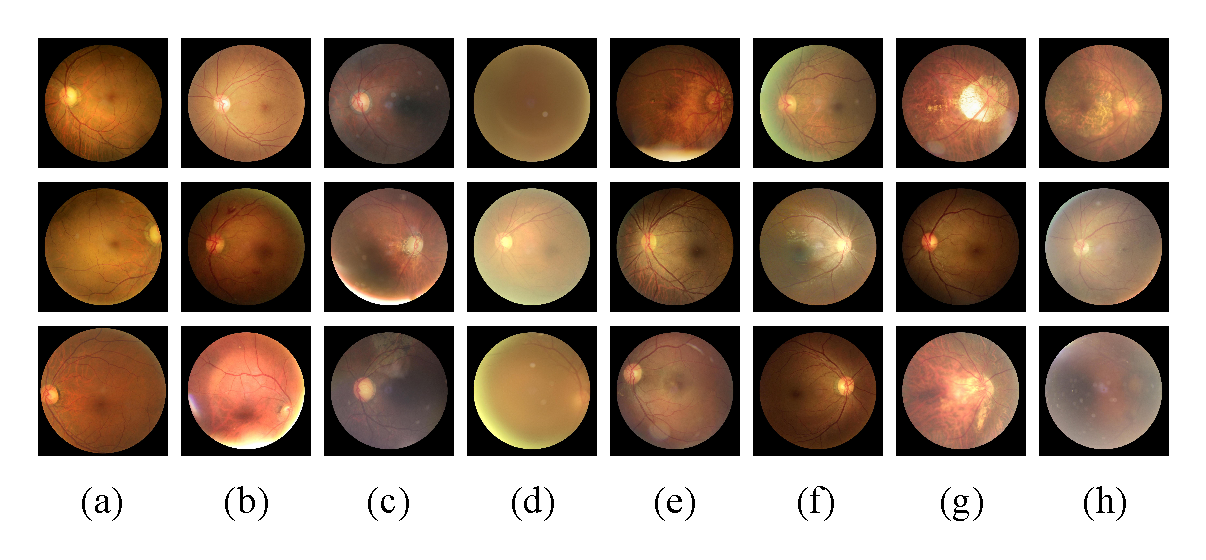
\includegraphics[width=0.86\textwidth]{./images/media/image5_padded.pdf}
\caption{ODIR 数据集中 8类眼底图像的示例样本，对应本文使用的 8个非互斥类别。其中(a)--(h)分别代表(a) 正常（N），(b) 糖尿病视网膜病变（D），(c) 青光眼（G），(d) 白内障（C），(e) 年龄相关性黄斑变性（A），(f) 高血压视网膜病变（H），(g) 病理性近视（M），(h) 其他异常（O）。 Example fundus images of the eight classes in the ODIR dataset, corresponding to the eight non-mutually exclusive classes used in this study. (a)--(h) denote (a) normal (N), (b) Diabetic Retinopathy (D), (c) Glaucoma (G), (d) Cataract (C), (e) Age-Related Macular Degeneration (A), (f) Hypertension (H), (g) Myopia (M), and (h) Others (O), respectively.}
\label{fig:odir-samples}
\end{figure}

为全面评估模型的域泛化能力，除 ODIR 域内泛化外，本文额外引入 RIADD 挑战赛提供的 RFMiD \hyperref[_Ref213949409]{{[}47{]}}数据集作为第一个独立跨域泛化数据集。RFMiD 包含3200张彩色眼底图像，训练集、验证集和测试集分别包含1920、640和640张图像，涵盖45种视网膜疾病或异常，由专业视网膜专家标注。其45类标签中含有部分与 ODIR 的8类标签重合的类别，这为模型泛化提供了基础。\figsubref{fig:rfmid-samples}{a}到\figsubref{fig:rfmid-samples}{h}选择性地展示了45种类别中的8类图像。考虑到 RFMiD 与 ODIR 的完整标签空间并不一致，本文选取二者共有的糖尿病视网膜病变（D）、年龄相关性黄斑变性（A）和病理性近视（M）三类进行跨域泛化。在该设置下，ODIR 侧构建得到1907张 D/A/M 三类训练图像，其中 D、A、M 的标签数分别为1425、255和253；RFMiD 侧使用验证集中的119张三类图像进行测试，其中 D、A、M 的标签数分别为83、24和21。

To comprehensively evaluate domain generalization capability, in addition to ODIR in-domain generalization, this study introduces RFMiD \hyperref[_Ref213949409]{{[}47{]}}, provided by the RIADD challenge, as the first independent cross-domain generalization dataset. RFMiD contains 3,200 color fundus images, with 1,920, 640, and 640 images in the training, validation, and test sets, respectively. It covers 45 retinal diseases or abnormalities annotated by professional retina specialists. Some of its 45 labels overlap with the eight labels in ODIR, providing a basis for model generalization. \hyperref[fig:rfmid-samples]{Fig.~\ref*{fig:rfmid-samples}.a} to \hyperref[fig:rfmid-samples]{Fig.~\ref*{fig:rfmid-samples}.h} show representative images from eight of the 45 categories. Since the complete label spaces of RFMiD and ODIR are inconsistent, this study selects their shared classes, Diabetic Retinopathy (D), Age-Related Macular Degeneration (A), and Myopia (M), for cross-domain generalization. Under this setting, 1,907 D/A/M training images are constructed on the ODIR side, with 1,425, 255, and 253 labels for D, A, and M, respectively. On the RFMiD side, 119 validation images from these three classes are used for testing, with 83, 24, and 21 labels for D, A, and M, respectively.

\begin{figure}[H]
\centering
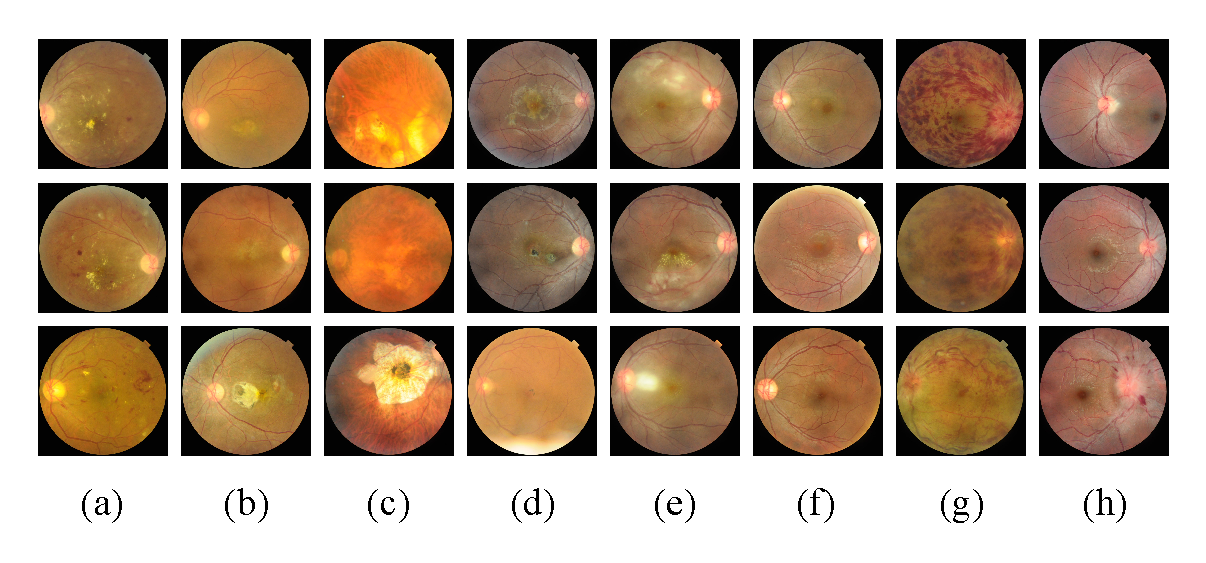
\includegraphics[width=0.86\textwidth]{./images/media/image6_padded.pdf}
\caption{RFMiD 数据集中选取的 8类眼底图像示例，其中(a)--(h)分别对应(a) 糖尿病视网膜病变（D），(b) 年龄相关性黄斑变性（A），(c) 近视（M），(d) 黄斑瘢痕（MS），(e) 视网膜炎（RS），(f) 中心性浆液性脉络膜视网膜病变（CSR），(g) 视网膜中央静脉阻塞（CRVO），(h) 视盘水肿（DE）。RFMiD 作为跨域泛化数据集使用，实验中与 ODIR 对齐后的共有标签空间为 D/A/M 三类，用于评估跨域泛化性能。 Examples of eight selected fundus image classes in the RFMiD dataset. (a)--(h) correspond to (a) Diabetic Retinopathy (D), (b) Age-Related Macular Degeneration (A), (c) Myopia (M), (d) Macular Scar (MS), (e) Retinitis (RS), (f) Central Serous Retinopathy (CSR), (g) Central Retinal Vein Occlusion (CRVO), and (h) Disc Edema (DE), respectively. RFMiD is used as a cross-domain generalization dataset. In the experiments, the shared label space aligned with ODIR consists of D/A/M classes and is used to evaluate cross-domain generalization performance.}
\label{fig:rfmid-samples}
\end{figure}

此外，本文引入来自于 Anawara Hamida 和 B.N.S.B. Zahurul Haque 眼科医院采集的 EDID \hyperref[_RefEDID2024]{{[}48{]}}数据集作为第二个独立跨域泛化数据集，以进一步验证所提方法在不同数据来源和不同标签组织方式下的泛化性能。EDID 原始数据共包含5335张眼底图像，覆盖10个单标签类别，包括中心性浆液性脉络膜视网膜病变、糖尿病视网膜病变、视盘水肿、青光眼、正常眼底、黄斑瘢痕、近视、翼状胬肉、视网膜脱离和视网膜色素变性，对应样本数分别为101、1509、127、1349、1024、444、500、17、125和139。\figsubref{fig:edid-samples}{a}到\figsubref{fig:edid-samples}{h}展示了 EDID 数据集中选取的8类典型眼底图像示例。

In addition, this study introduces the EDID \hyperref[_RefEDID2024]{{[}48{]}} dataset collected from Anawara Hamida and B.N.S.B. Zahurul Haque Eye Hospital as the second independent cross-domain generalization dataset, further validating the generalization performance of the proposed method across different data sources and label organizations. The original EDID dataset contains 5,335 fundus images covering 10 single-label classes, including Central Serous Retinopathy, Diabetic Retinopathy, Disc Edema, Glaucoma, normal, Macular Scar, Myopia, Pterygium, Retinal Detachment, and Retinitis Pigmentosa, with 101, 1,509, 127, 1,349, 1,024, 444, 500, 17, 125, and 139 samples, respectively. \hyperref[fig:edid-samples]{Fig.~\ref*{fig:edid-samples}.a} to \hyperref[fig:edid-samples]{Fig.~\ref*{fig:edid-samples}.h} show examples of eight representative fundus image classes selected from EDID.

\begin{figure}[H]
\centering
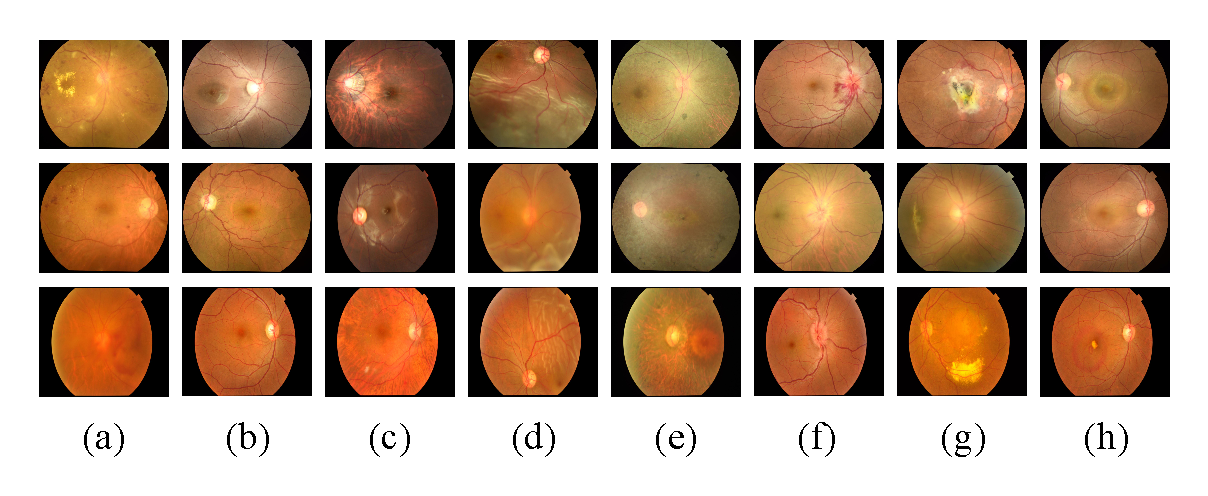
\includegraphics[width=0.86\textwidth]{./images/media/edid_samples_padded.pdf}
\caption{EDID 数据集中选取的 8类眼底图像示例，其中(a)--(h)分别对应(a) 糖尿病视网膜病变（D），(b) 青光眼（G），(c) 近视（M），(d) 视网膜脱离（RD），(e) 视网膜色素变性（RP），(f) 视盘水肿（DE），(g) 黄斑瘢痕（MS），(h) 中心性浆液性脉络膜视网膜病变（CSR）。EDID 为单标签跨域泛化数据集，实验中与 ODIR 对齐后的共有标签空间为 D/G/M 三类，用于评估不同数据来源和标签组织方式下的泛化性能。 Examples of eight selected fundus image classes in the EDID dataset. (a)--(h) correspond to (a) Diabetic Retinopathy (D), (b) Glaucoma (G), (c) Myopia (M), (d) Retinal Detachment (RD), (e) Retinitis Pigmentosa (RP), (f) Disc Edema (DE), (g) Macular Scar (MS), and (h) Central Serous Retinopathy (CSR), respectively. EDID is used as a single-label cross-domain generalization dataset. In the experiments, the shared label space aligned with ODIR consists of D/G/M classes and is used to evaluate generalization performance under different data sources and label organizations.}
\label{fig:edid-samples}
\end{figure}

与 RFMiD 类似，考虑到 EDID 与 ODIR 的完整标签空间并不一致，本文选取二者共有的糖尿病视网膜病变（D）、青光眼（G）和病理性近视（M）三类构建跨域泛化数据集，共得到3358张图像，其中 D、G、M 的样本数分别为1509、1349和500。由于 EDID 为单标签数据集，本文将其视为多标签识别任务中的一种特殊情形，即每张图像仅有一个阳性标签，并在 D/G/M 三类空间下进行跨域泛化评估。相应地，在 ODIR 侧构建 D/G/M 三类训练子集，共包含1871张图像，其中 D、G、M 的样本数分别为1401、227和243。

Similar to RFMiD, since the complete label spaces of EDID and ODIR are inconsistent, this study selects their shared classes, Diabetic Retinopathy (D), Glaucoma (G), and Myopia (M), to construct a cross-domain generalization dataset with 3,358 images, including 1,509, 1,349, and 500 samples for D, G, and M, respectively. Since EDID is a single-label dataset, it is treated as a special case of the multi-label recognition task, where each image has only one positive label, and cross-domain generalization is evaluated in the D/G/M three-class space. Correspondingly, a D/G/M training subset is constructed on the ODIR side, containing 1,871 images, with 1,401, 227, and 243 samples for D, G, and M, respectively.

\letteredsubsection{B. 实验设置}

\letteredsubsection{B. Experimental Settings}

所有实验均以 ResNet50 作为骨干网络，并在 PyTorch 框架下实现。评估指标沿用 ODIR 官方标准：Kappa 系数、F1、AUC 以及三者平均值 Final score。Kappa 阈值固定为0.5，F1 采用 micro 平均方式以缓和类别不平衡影响。

All experiments use ResNet50 as the backbone and are implemented in PyTorch. The evaluation metrics follow the official ODIR standard: Kappa, F1, AUC, and their average value, Final score. The Kappa threshold is fixed at 0.5, and F1 uses micro averaging to alleviate the influence of class imbalance.

对于基线模型，我们参考 ODIR 原始的 ResNet50 的实现，并在此基础上进行了改进：原论文采用双目样本成对输入，尝试不同的特征层融合策略（如 concat、prod、sum）后接8个独立的分类头进行患者级预测。而我们改为以单目图像为输入样本，样本同时带有所属患者的编号，分类器统一为单个多标签分类头，输出8维 logits 后经 Sigmoid 激活得到各疾病概率，损失函数为标准二元交叉熵（BCE）。推理阶段，将同一患者左右眼的单目预测结果按逻辑合并得到患者级预测，从而与官方指标完全对齐。该改进避免了特征融合带来的噪声放大和个体差异信息稀释，尤其在双目病变程度不一致时更有优势。

For the baseline, we follow the original ResNet50 implementation of ODIR and modify it for our setting. The original paper uses paired binocular samples as input, evaluates different feature-level fusion strategies such as concat, prod, and sum, and then uses eight independent classification heads for patient-level prediction. In contrast, we use monocular images as input samples, with each sample carrying its corresponding patient identifier. The classifier is implemented as a single multi-label classification head, which outputs eight-dimensional logits and obtains disease probabilities through Sigmoid activation. The loss function is standard binary cross entropy (BCE). During inference, monocular predictions from the left and right eyes of the same patient are logically merged to obtain patient-level predictions, fully aligning with the official metrics. This modification avoids noise amplification caused by feature fusion and dilution of individual-difference information, and is especially advantageous when disease severity differs between the two eyes.

训练配置如下：优化器选择 Adam，初始学习率\(4 \times 10^{-7}\)，采用 OneCycleLR 调度策略（前10\%轮次从初始学习率线性升温至峰值\(1 \times 10^{-5}\)，有助于模型快速跳出局部最优，后90\%轮次退火，有助于收敛和找到更优解），训练 epoch 为50，batch size 为32，输入分辨率为448×448。所提方法在2张 RTX 4080 Super 上完成训练。后续实验结果表明，我们的改进基线模型（Off-site 双目 Final score 76.19）比起 ODIR 原文 ResNet50 实现（Off-site 双目 Final score 68.00）能达到更好的效果。

The training configuration is as follows. Adam is used as the optimizer, with an initial learning rate of \(4 \times 10^{-7}\). OneCycleLR is adopted as the scheduling strategy: the learning rate linearly warms up from the initial learning rate to the peak value of \(1 \times 10^{-5}\) during the first 10\% of epochs to help the model quickly escape local optima, and then anneals during the remaining 90\% of epochs to facilitate convergence and reach a better solution. The number of training epochs is 50, the batch size is 32, and the input resolution is \(448 \times 448\). The proposed method is trained on two RTX 4080 Super GPUs. Experimental results show that our improved baseline model, with an Off-site binocular Final score of 76.19, outperforms the ResNet50 implementation in the original ODIR paper, which reports an Off-site binocular Final score of 68.00.

\letteredsubsection{C. 与现有方法对比}

\letteredsubsection{C. Comparison with Existing Methods}

为评估所提方法在 ODIR 数据集上的识别性能，我们选取了四个公开发表的多标签眼科疾病识别方法进行对比，包括 ODIR 数据集论文提供的官方基线（Li et al. \hyperref[_Ref213949402]{{[}46{]}}）以及三项后续在该数据集上报告结果的工作（Gour and Khanna \hyperref[_Ref214903299]{{[}49{]}}、He et al. \hyperref[_Ref213950338]{{[}20{]}}、Ou et al. \hyperref[_Ref214903327]{{[}50{]}}）。这些方法主要聚焦于提升 Final score，未考虑跨域泛化或隐私保护。

To evaluate the recognition performance of the proposed method on the ODIR dataset, we compare it with four published multi-label ocular disease recognition methods, including the official baseline provided in the ODIR dataset paper by Li et al. \hyperref[_Ref213949402]{{[}46{]}} and three subsequent works reporting results on this dataset by Gour and Khanna \hyperref[_Ref214903299]{{[}49{]}}, He et al. \hyperref[_Ref213950338]{{[}20{]}}, and Ou et al. \hyperref[_Ref214903327]{{[}50{]}}. These methods mainly focus on improving Final score and do not consider cross-domain generalization or privacy preservation.

Gour and Khanna \hyperref[_Ref214903299]{{[}49{]}}提出基于转移学习的 CNN 框架，骨干网络采用 VGG16，通过数据增强方法扩充 ODIR 数据集，然后采用 SGD 优化器细调模型，焦点在于利用预训练权重捕捉血管、视盘、黄斑等结构异常，以提升多类共存场景的识别性能。

Gour and Khanna \hyperref[_Ref214903299]{{[}49{]}} proposed a transfer-learning-based CNN framework with VGG16 as the backbone. The ODIR dataset is expanded through data augmentation, and the model is fine-tuned using the SGD optimizer. The method uses pretrained weights to capture structural abnormalities involving vessels, optic discs, and maculae, thereby improving recognition performance in multi-class co-occurrence scenarios.

He et al. \hyperref[_Ref213950338]{{[}20{]}}开发密集相关网络（DCNet），包括骨干 CNN 提取双目特征、空间相关模块捕捉像素级相关性，以及分类器生成患者级分类结果。核心原理是通过密集卷积块融合双目特征，建模 DR 与 AMD 等疾病共现，但需依赖双目输入。

He et al. \hyperref[_Ref213950338]{{[}20{]}} developed a dense correlation network (DCNet), which includes a backbone CNN for extracting binocular features, a spatial correlation module for capturing pixel-level relevance, and a classifier for generating patient-level classification results. Its core idea is to fuse binocular features through dense convolutional blocks and model disease co-occurrence such as DR and AMD, but it relies on binocular input.

Ou et al. \hyperref[_Ref214903327]{{[}50{]}}设计双流交互 CNN（BFENet），使用特征增强模块通过注意力机制捕捉双目局部-全局依赖，并通过多尺度模块叠加不同分辨率特征以丰富表示。其原理在于利用双流交互强化病变区域（如微血管瘤、出血点），提升多标签识别性能，但未考虑隐私或跨域场景。

Ou et al. \hyperref[_Ref214903327]{{[}50{]}} designed a two-stream interactive CNN (BFENet). A feature enhancement module captures local-global binocular dependencies through an attention mechanism, and a multi-scale module aggregates features at different resolutions to enrich representations. The method enhances lesion regions, such as microaneurysms and hemorrhages, through two-stream interaction to improve multi-label recognition performance, but it does not consider privacy or cross-domain scenarios.

\tabref{tab:sota-compare}与\figref{fig:sota-compare}报告了 Off-site test 和 On-site test 集上的双目指标对比。对比结果显示，所提方法在 Off-site 的 Final score 为78.85，领先 BFENet \hyperref[_Ref214903327]{{[}50{]}} 0.85；在 On-site 为77.49，领先 BFENet \hyperref[_Ref214903327]{{[}50{]}} 0.79。该结果证明了双分支引导特征学习与自适应标签-特征关联性构建在 ODIR 多标签识别任务中的有效性。

\hyperref[tab:sota-compare]{Table~\ref*{tab:sota-compare}} and \hyperref[fig:sota-compare]{Fig.~\ref*{fig:sota-compare}} compare binocular metrics on the Off-site test and On-site test sets. The proposed method achieves a Final score of 78.85 on Off-site, outperforming BFENet \hyperref[_Ref214903327]{{[}50{]}} by 0.85, and achieves 77.49 on On-site, outperforming BFENet \hyperref[_Ref214903327]{{[}50{]}} by 0.79. These results demonstrate the effectiveness of dual-branch guided feature learning and adaptive label-feature relevance construction on the ODIR multi-label recognition task.

% Chapter 4 Experiments - Table 2
% Comparison with existing methods on Off-site and On-site.
\begin{table}[!htb]
\centering
\caption{与现有方法在 ODIR Off-site 和 On-site 上的双目指标对比。红色表示各指标中的最优结果，蓝色表示次优结果。与 BFENet \hyperref[_Ref214903327]{{[}50{]}} 相比，所提方法虽然在 F1 和 AUC 两项指标上略低，但在 Kappa 上提升更明显，并在两个测试集上的 Final score 均取得了最优结果。 Comparison of binocular metrics with existing methods on ODIR Off-site and On-site. Red denotes the best result for each metric, and blue denotes the second-best result. Compared with BFENet \hyperref[_Ref214903327]{{[}50{]}}, the proposed method is slightly lower in F1 and AUC, but achieves a more obvious improvement in Kappa and obtains the best Final score on both test sets.}
\label{tab:sota-compare}
\resizebox{\textwidth}{!}{
\begin{tabular}{lcccccccc}
\toprule
\multirow{2}{*}{Method} & \multicolumn{4}{c}{Off-site} & \multicolumn{4}{c}{On-site} \\
\cmidrule(lr){2-5}\cmidrule(lr){6-9}
& Kappa & F1 & AUC & Final & Kappa & F1 & AUC & Final \\
\midrule
Li et al. \hyperref[_Ref213949402]{{[}46{]}} & 35.45 & 84.83 & 83.72 & 68.00 & 36.97 & 85.35 & 84.08 & 68.80 \\
Gour and Khanna \hyperref[_Ref214903299]{{[}49{]}} & 43.30 & 85.30 & 84.90 & 71.20 & 42.00 & 84.90 & 83.40 & 70.10 \\
He et al. \hyperref[_Ref213950338]{{[}20{]}} & 52.00 & 88.60 & 90.30 & 77.00 & 50.00 & 87.70 & 89.70 & 75.80 \\
BFENet \hyperref[_Ref214903327]{{[}50{]}} & \textcolor{blue}{53.50} & \textcolor{red}{89.20} & \textcolor{red}{91.20} & \textcolor{blue}{78.00} & \textcolor{blue}{51.30} & \textcolor{red}{88.60} & \textcolor{red}{90.30} & \textcolor{blue}{76.70} \\
Ours & \textcolor{red}{57.05} & \textcolor{blue}{89.03} & \textcolor{blue}{90.48} & \textcolor{red}{78.85} & \textcolor{red}{54.03} & \textcolor{blue}{88.38} & \textcolor{blue}{90.07} & \textcolor{red}{77.49} \\
\bottomrule
\end{tabular}
}
\end{table}


\begin{figure}[H]
\centering
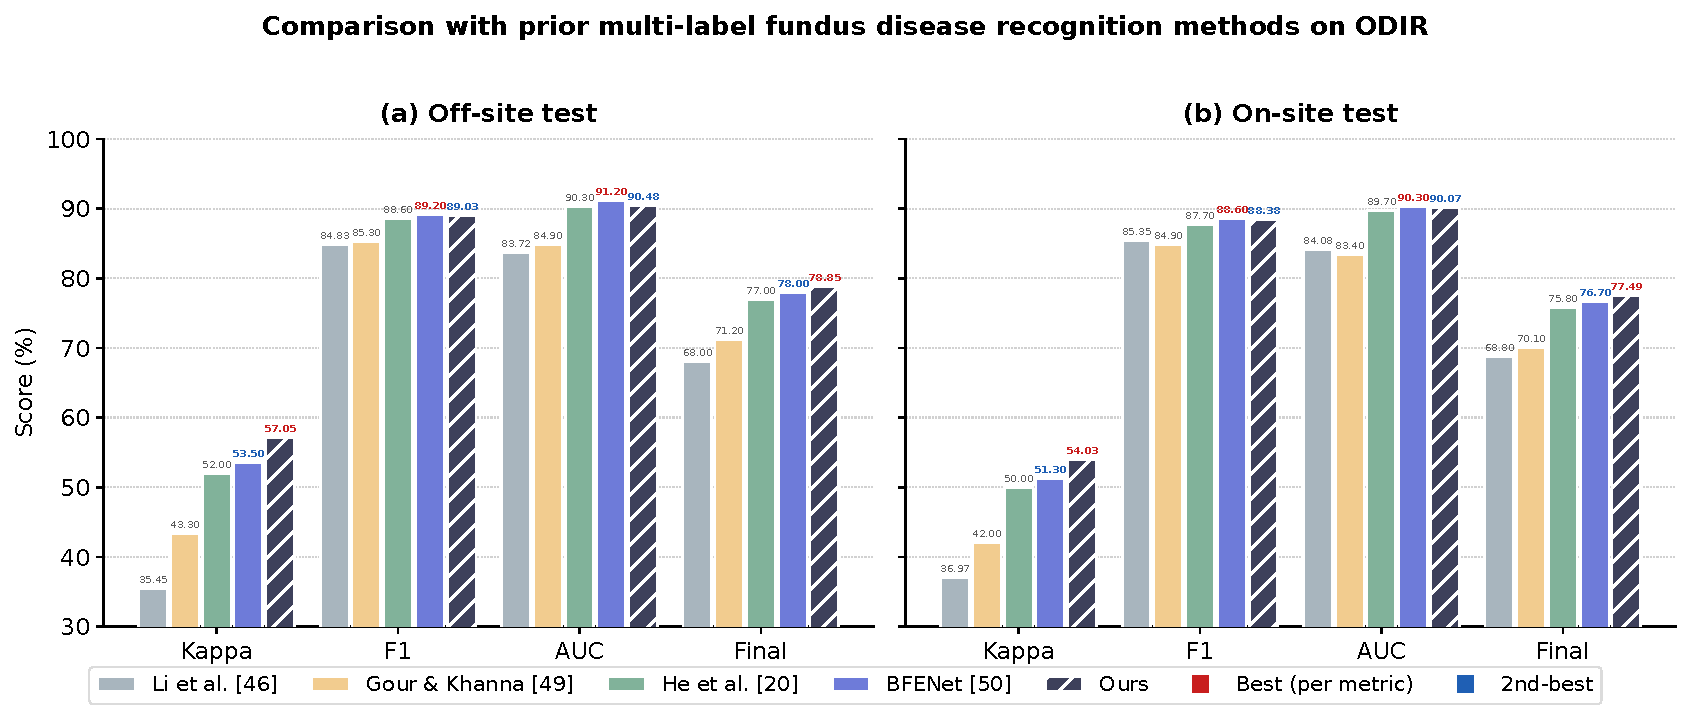
\includegraphics[width=0.96\textwidth]{./images/plots/fig_sota_compare.pdf}
\caption{与现有方法在 ODIR 上的指标对比可视化，(a) Off-site test 与 (b) On-site test 分别对应\tabref{tab:sota-compare}中的两组双目指标。柱状图按 Kappa、F1、AUC 和 Final score 四项指标分组，各指标中红色数值标注最优结果、蓝色标注次优结果。所提方法（Ours）在两个测试集的 Kappa 与 Final score 上均取得最优。 Visual comparison of metrics with existing methods on ODIR, where (a) Off-site test and (b) On-site test correspond to the two groups of binocular metrics in \hyperref[tab:sota-compare]{Table~\ref*{tab:sota-compare}}. The bars are grouped by the four metrics Kappa, F1, AUC, and Final score; within each metric, red values mark the best result and blue values mark the second-best. The proposed method (Ours) achieves the best Kappa and Final score on both test sets.}
\label{fig:sota-compare}
\end{figure}

需要指出的是，现有对比方法主要围绕 ODIR 内部多标签识别指标进行优化，较少同时考虑域泛化和隐私保护。相比之下，本文除在 ODIR Off-site 和 On-site 上取得更高 Final score 外，还在 RFMiD 和 EDID 两个跨域泛化数据集上验证了未知域性能，并进一步评估隐私保护训练下的性能衰减。上述结果共同说明，所提方法不仅追求单一数据集上识别性能，也面向更贴近临床部署的数据共享受限和隐私保护场景。

Existing comparison methods mainly optimize internal multi-label recognition metrics on ODIR and rarely consider domain generalization and privacy preservation simultaneously. In contrast, in addition to achieving higher Final scores on ODIR Off-site and On-site, this study validates unseen-domain performance on two cross-domain generalization datasets, RFMiD and EDID, and further evaluates performance degradation under privacy-preserving training. These results indicate that the proposed method is not limited to improving recognition performance on a single dataset, but is also designed for clinically relevant settings where data sharing is restricted and privacy preservation is required.

\letteredsubsection{D. 消融实验结果}

\letteredsubsection{D. Ablation Study Results}

为系统验证所提方法中两大核心模块，即双分支引导域不变特征提取（DFE）与自适应标签-特征关联性构建（ARC）的独立贡献及协同增益，同时考察 CAM 引导对模型可解释性的提升，我们在 ODIR Off-site 双目指标上进行了逐模块消融实验，结果如\tabref{tab:ablation}所示，并在\figref{fig:ablation-radar}中以雷达图直观对比各模型的指标分布。\tabref{tab:ablation}同时给出单目与双目两组指标，二者呈现一致的提升趋势；为与官方患者级评估标准对齐、并保持正文简洁，下文仅就双目指标展开分析。

To assess the independent contributions and synergistic gains of the two core modules in the proposed method, namely Dual-Branch Guided Domain-Invariant Feature Extraction (DFE) and Adaptive Label-Feature Relevance Construction (ARC), and to examine the improvement in model interpretability brought by CAM guidance, we conduct module-wise ablation experiments using ODIR Off-site metrics. The results are shown in \hyperref[tab:ablation]{Table~\ref*{tab:ablation}}, and \hyperref[fig:ablation-radar]{Fig.~\ref*{fig:ablation-radar}} provides an intuitive radar-chart comparison of the metric distributions across models. \hyperref[tab:ablation]{Table~\ref*{tab:ablation}} reports both monocular and binocular metrics, which show a consistent improvement trend; to align with the official patient-level evaluation standard and keep the main text concise, the following analysis focuses on the binocular metrics.

\input{manuscripts/compare/tables/src/table6_ablation_compare.tex}

\begin{figure}[H]
\centering
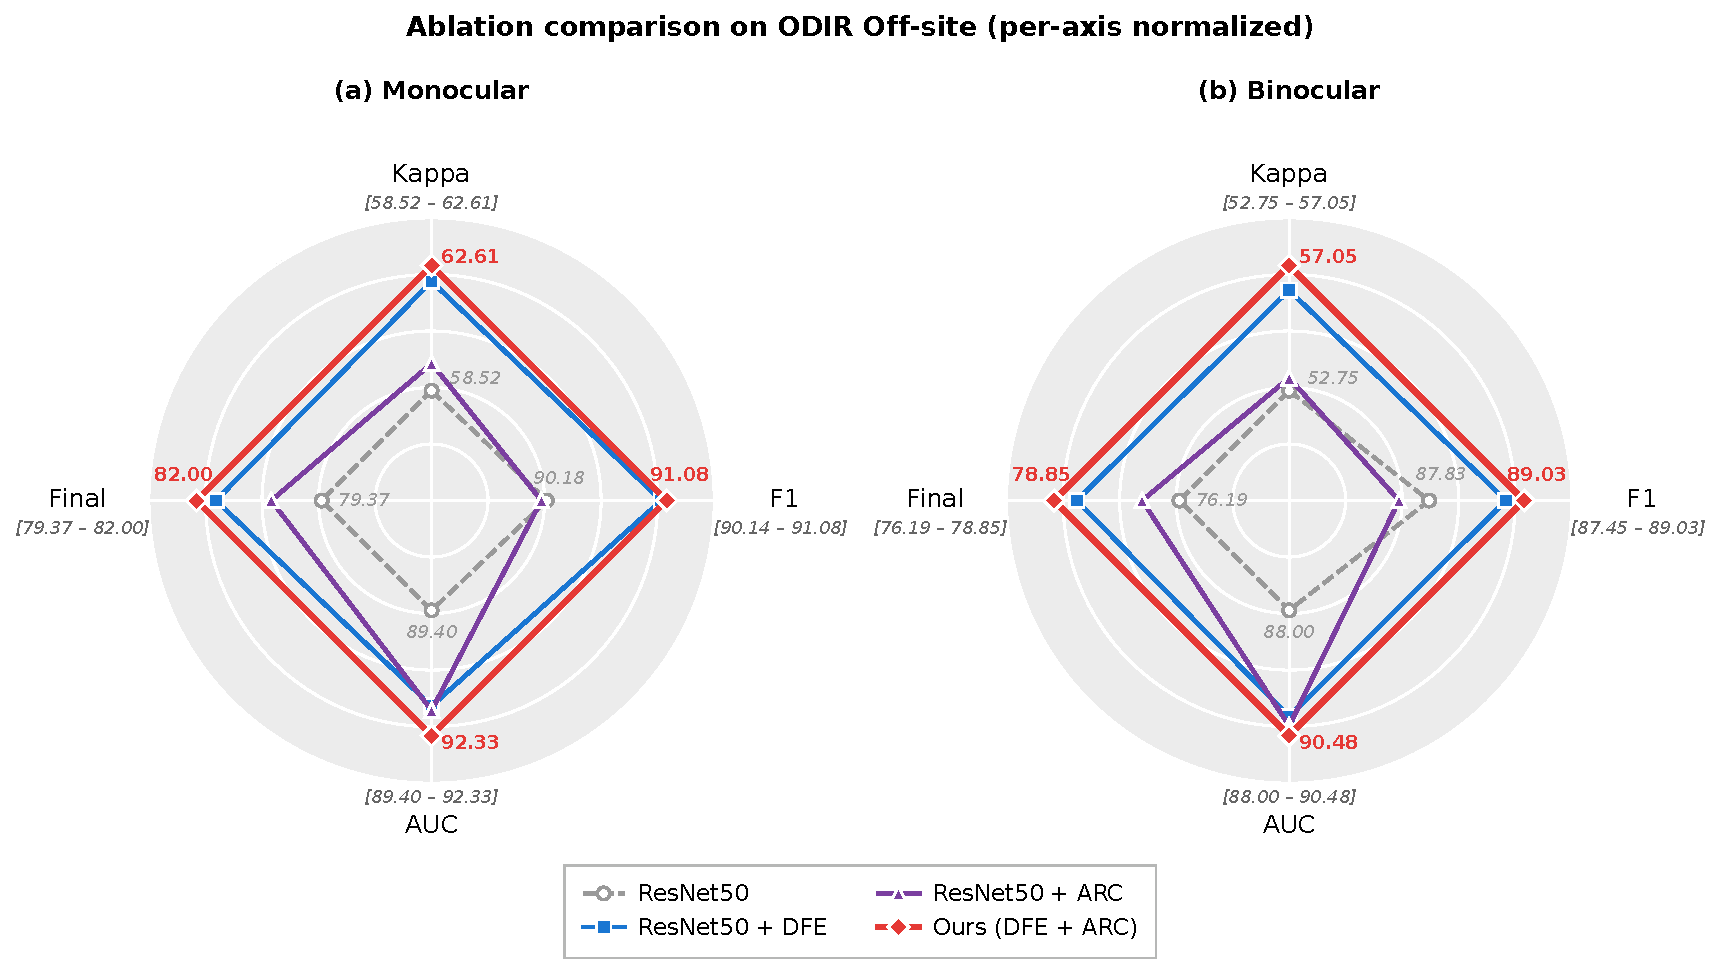
\includegraphics[width=0.92\textwidth]{./images/plots/fig_ablation_radar.pdf}
\caption{消融实验中各模型在 ODIR Off-site 上的指标雷达图，分别给出 (a) 单目（Monocular）与 (b) 双目（Binocular）两种评估方式下的结果，二者均与\tabref{tab:ablation}一致。每个轴对应一项指标（Kappa、F1、AUC、Final），并按该轴取值范围独立归一化以放大模型间差异，多边形越向外表示指标越高。所提方法（Ours）在各项指标上整体外扩，优于仅引入 DFE 或 ARC 的变体及基线。 Radar charts of the metrics of each model on ODIR Off-site in the ablation study, showing the results under (a) monocular and (b) binocular evaluation protocols, both consistent with \hyperref[tab:ablation]{Table~\ref*{tab:ablation}}. Each axis corresponds to one metric (Kappa, F1, AUC, Final) and is independently normalized according to the value range of that axis to amplify differences among models; the further the polygon extends outward, the higher the metric. The proposed method (Ours) expands outward on all metrics overall, outperforming the variants that introduce only DFE or only ARC as well as the baseline.}
\label{fig:ablation-radar}
\end{figure}

\begin{itemize}
\item
  ResNet50：仅使用单分支 ResNet50 与标准多标签分类头，Final score 为76.19，Kappa 为52.75，AUC 是88.00。

  ResNet50: only a single-branch ResNet50 and a standard multi-label classification head are used. The Final score is 76.19, Kappa is 52.75, and AUC is 88.00.
\item
  ResNet50+DFE：仅引入完整的双分支引导域不变特征提取模块，Final score 提升至78.37（+2.18），Kappa 提升3.45，AUC 提升2.10。性能提升主要源于 CAM 引导残差加权与掩码机制有效抑制了域特定噪声，使模型更关注域不变特征，是整体性能提升的重要来源。

  ResNet50+DFE: only the complete Dual-Branch Guided Domain-Invariant Feature Extraction module is introduced. The Final score increases to 78.37 (+2.18), Kappa increases by 3.45, and AUC increases by 2.10. The improvement mainly comes from CAM-guided residual weighting and the mask mechanism, which effectively suppress domain-specific noise and encourage the model to focus on domain-invariant features.

\item
  ResNet50+ARC：仅引入自适应标签-特征关联性构建模块，Final score 提升至76.98（+0.79），Kappa 提升0.44，AUC 提升2.29。该模块通过显式建模疾病共现依赖（如 DR 与 AMD、近视与视盘异常）降低了漏检率，多标签识别性能提高。

  ResNet50+ARC: only the Adaptive Label-Feature Relevance Construction module is introduced. The Final score increases to 76.98 (+0.79), Kappa increases by 0.44, and AUC increases by 2.29. By explicitly modeling disease co-occurrence dependencies, such as DR and AMD or Myopia and optic-disc abnormalities, this module reduces the false-negative rate and improves multi-label recognition performance.
\item
  ResNet50+DFE+ARC（所提方法，ours）：同时启用两大模块协同后，Final score 进一步升至78.85（较基线+2.66），Kappa 达到57.05（+4.30），F1 与 AUC 分别达到89.03（+1.20）和90.48（+2.48）。总增益与两模块独立增益之和接近（2.66 ≈ 2.18+0.79=2.97），说明两模块功能互补、组合时无明显冲突：DFE 为 ARC 提供更稳定的域不变特征，使 Transformer 能更精准地学习标签-标签关联性与标签-特征关联性；ARC 的注意力一致性损失反过来进一步约束双分支输出分布，提升特征表示的稳定性。进一步从\figref{fig:cam-visualization}的可视化结果可以看出，相比 baseline，所提方法得到的 CAM，其模型关注区域对图像边缘、光照伪影的响应减少，更收敛到眼球、血管等疾病相关区域，模型可解释性增强。

  ResNet50+DFE+ARC (the proposed method, ours): when both modules are enabled, the Final score further increases to 78.85 (+2.66 over the baseline), Kappa reaches 57.05 (+4.30), and F1 and AUC reach 89.03 (+1.20) and 90.48 (+2.48), respectively. The total gain is close to the sum of the individual gains of the two modules (\(2.66 \approx 2.18 + 0.79 = 2.97\)), indicating that the two modules are functionally complementary and exhibit no obvious conflict when combined. DFE provides more stable domain-invariant features for ARC, enabling Transformer to learn label-label relevance and label-feature relevance more accurately. Conversely, the attention consistency loss of ARC further constrains the output distributions of the two branches and improves feature stability. In addition, the visualization results in \hyperref[fig:cam-visualization]{Fig.~\ref*{fig:cam-visualization}} show that, compared with the baseline, the CAMs obtained by the proposed method respond less to image edges and illumination artifacts, and the model-attended regions concentrate more on the eyeball, vessels, and other disease-related regions, indicating enhanced model interpretability.
\end{itemize}

\begin{figure}[H]
\centering
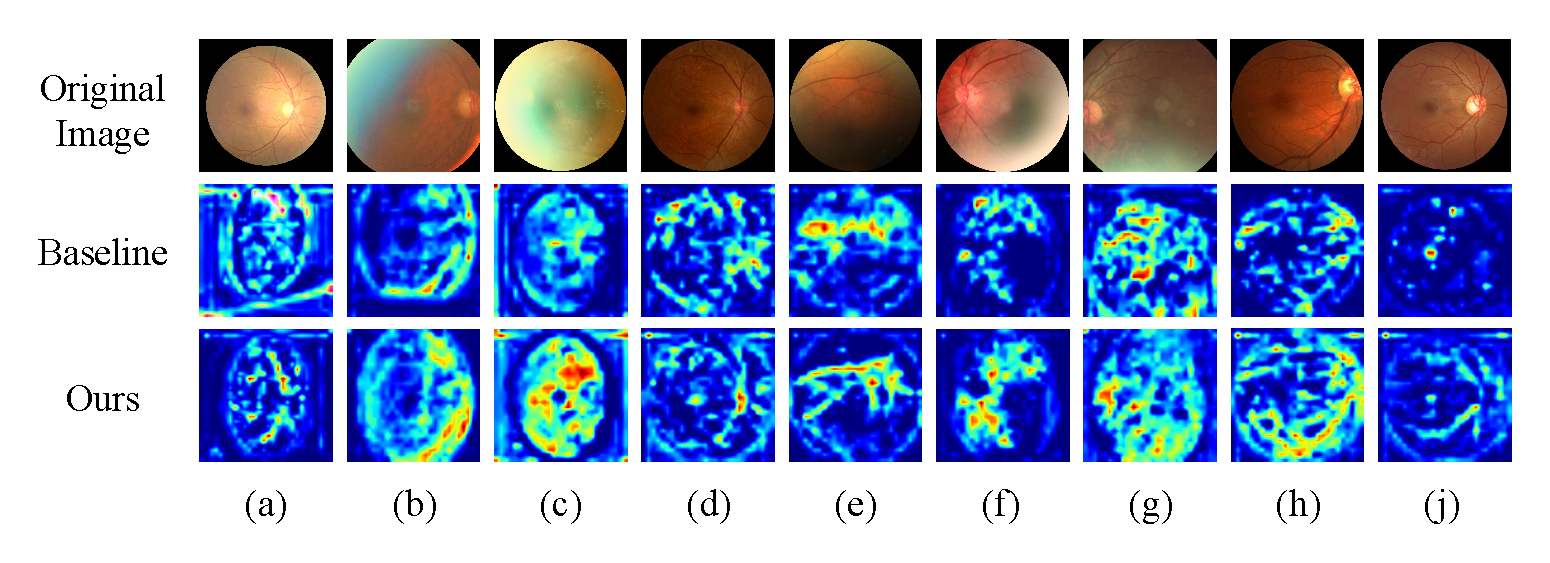
\includegraphics[width=0.92\textwidth]{./images/media/image8_padded.pdf}
\caption{基线方法与所提方法在 ODIR Off-site 部分样本上的 CAM 模型关注区域可视化对比，其中(a)--(j) 为不同测试样本。相比基线模型，所提方法的模型关注区域更集中于眼球、血管和疾病相关区域，对图像边缘、光照伪影等无关背景的响应更弱，说明所提方法能够有效抑制域特定噪声并增强可解释性。 Comparison of CAM-based model-attended region visualizations between the baseline and the proposed method on selected ODIR Off-site samples, where (a)--(j) denote different test samples. Compared with the baseline, the model-attended regions of the proposed method are more concentrated on the eyeball, vessels, and disease-related regions, with weaker responses to irrelevant background factors such as image edges and illumination artifacts. This indicates that the proposed method effectively suppresses domain-specific noise and enhances interpretability.}
\label{fig:cam-visualization}
\end{figure}

消融结果证明：自适应标签-特征关联性构建（ARC）验证了标签关联建模对多疾病共存场景的有效性，双分支引导域不变特征提取（DFE）验证了在多机构联合训练难以满足时，仅利用单一源域学习域不变特征的必要性。两模块的深度融合协同使得所提方法在仅使用单一源域训练的情况下进一步提升多标签识别性能，并为后续跨域泛化结果提供支撑，体现了本方法设计的科学性与高效性。

The ablation results show that Adaptive Label-Feature Relevance Construction (ARC) improves label relevance modeling in multi-disease co-occurrence scenarios, while Dual-Branch Guided Domain-Invariant Feature Extraction (DFE) supports learning domain-invariant features from a single source domain when multi-institutional joint training is restricted. The integration of the two modules further improves multi-label recognition performance under single-source-domain training and provides a basis for the subsequent cross-domain generalization results.

\letteredsubsection{E. 泛化性能结果}

\letteredsubsection{E. Generalization Performance Results}

为全面验证所提方法在单一源域训练条件下的泛化能力以及隐私保护机制的有效性，我们按照"域内泛化 \(\rightarrow\) 跨域泛化 \(\rightarrow\) 隐私保护"的递进逻辑组织评估：首先在 ODIR 域内（Off-site 与 On-site）验证多标签识别性能，再在 RFMiD 与 EDID 两个未知域上考察跨域泛化能力，最后评估引入隐私保护机制后的性能保留情况。其中前两步在非隐私保护条件下完成，第三步在隐私保护条件下完成。

To comprehensively validate the generalization capability of the proposed method under single-source-domain training and the effectiveness of the privacy-preserving mechanism, we organize the evaluation in three stages: in-domain generalization, cross-domain generalization, and privacy preservation. We first validate multi-label recognition performance within the ODIR domain (Off-site and On-site), then examine cross-domain generalization capability on the two unseen domains RFMiD and EDID, and finally evaluate the performance retention after introducing the privacy-preserving mechanism. The first two stages are completed under the non-private setting, while the third stage is completed under the privacy-preserving setting.


1. 非隐私保护条件下的泛化性能 结果如\tabref{tab:generalization}所示，表中报告了基线模型与所提方法在不同测试集上的 Final score。泛化实验按三个评估方向组织：ODIR 域内的 Off-site \(\rightarrow\) On-site、ODIR 到 RFMiD 的跨域泛化，以及 ODIR 到 EDID 的跨域泛化。每个方向均基于训练过程中保存的前5个候选检查点进行模型选择与评估，即分别在基线模型和所提方法的候选检查点中确定测试集表现最优的一组检查点，并同步报告该组检查点在源域 Off-site 和目标域上的结果。

1. Generalization performance under the non-private setting. The results are shown in \hyperref[tab:generalization]{Table~\ref*{tab:generalization}}, which reports the Final scores of the baseline and the proposed method on different test sets. The generalization experiments are organized along three evaluation directions: ODIR in-domain Off-site \(\rightarrow\) On-site, cross-domain generalization from ODIR to RFMiD, and cross-domain generalization from ODIR to EDID. For each direction, model selection and evaluation are based on the top five candidate checkpoints saved during training. Specifically, the checkpoint group with the best test-set performance is selected from the candidate checkpoints of the baseline and the proposed method, respectively, and the results of this checkpoint group on the source-domain Off-site set and the target domain are reported simultaneously.

% Chapter 4 Experiments - Table 4
% Generalization performance on ODIR, RFMiD/RIADD, and EDID.
\begin{table}[!htb]
\centering
\caption{不同测试集上的泛化性能比较。比较了基线模型与所提方法在 ODIR 域内泛化（Off-site $\rightarrow$ On-site）以及 ODIR 到 RFMiD、EDID 跨域泛化中的表现，比较的指标均为Final score。其中，Off-site $\rightarrow$ On-site 同时报告了单目与双目结果，跨域泛化部分报告了各数据集对齐三类标签空间后的单目结果；每个方向均在候选检查点中选择测试集表现最优的模型进行报告。总体上，所提方法在各测试方向上均优于基线模型。 Comparison of generalization performance on different test sets. The table compares the baseline and the proposed method on ODIR in-domain generalization (Off-site $\rightarrow$ On-site) and cross-domain generalization from ODIR to RFMiD and EDID, using Final score as the metric. Off-site $\rightarrow$ On-site reports both monocular and binocular results, while cross-domain generalization reports monocular results after aligning each dataset to a three-class label space. For each direction, the checkpoint with the best test-set performance is selected from candidate checkpoints. Overall, the proposed method outperforms the baseline in all evaluation directions.}
\label{tab:generalization}
\resizebox{\textwidth}{!}{
\begin{tabular}{lcccccccc}
\toprule
\multirow{3}{*}{Model} & \multicolumn{4}{c}{Off-site $\rightarrow$ On-site} & \multicolumn{2}{c}{Off-site $\rightarrow$ RFMiD} & \multicolumn{2}{c}{Off-site $\rightarrow$ EDID} \\
\cmidrule(lr){2-5}\cmidrule(lr){6-7}\cmidrule(lr){8-9}
& \multicolumn{2}{c}{Off-site} & \multicolumn{2}{c}{On-site} & Off-site & RFMiD & Off-site & EDID \\
\cmidrule(lr){2-3}\cmidrule(lr){4-5}\cmidrule(lr){6-7}\cmidrule(lr){8-9}
& Monocular & Binocular & Monocular & Binocular & Monocular & Monocular & Monocular & Monocular \\
\midrule
ResNet50 & 79.37 & 76.19 & 77.30 & 75.23 & 94.39 & 83.86 & 94.30 & 52.16 \\
\textbf{Ours} & \textbf{81.71} & \textbf{78.79} & \textbf{78.98} & \textbf{77.49} & \textbf{95.94} & \textbf{85.06} & \textbf{96.03} & \textbf{55.35} \\
\bottomrule
\end{tabular}
}
\end{table}


在 ODIR 域内泛化中，测试集为 On-site，\tabref{tab:generalization}同时报告单目（Monocular）和双目（Binocular）两种评估方式。基线模型对应检查点在 Off-site 和 On-site 上的双目指标分别为76.19和75.23，而所提方法对应检查点将指标提升至78.79和77.49，增幅分别达2.60和2.26个百分点；单目指标同样由79.37和77.30提升至81.71和78.98。这说明双分支引导特征学习与 CAM 引导注意力能够增强模型对疾病相关区域的关注。其中双目指标低于单目指标的原因是，模型本身以单目数据进行训练，推理阶段将同一患者左右眼预测结果合并时，任一只眼的错误预测都可能影响患者级判断，从而放大单目小错误对最终指标的影响。

For ODIR in-domain generalization, the test set is On-site, and \hyperref[tab:generalization]{Table~\ref*{tab:generalization}} reports both monocular and binocular evaluation protocols. The baseline checkpoint achieves binocular scores of 76.19 and 75.23 on Off-site and On-site, respectively, whereas the corresponding checkpoint of the proposed method improves these scores to 78.79 and 77.49, with gains of 2.60 and 2.26 percentage points. The monocular metrics also increase from 79.37 and 77.30 to 81.71 and 78.98. This indicates that dual-branch guided feature learning and CAM-guided attention can enhance the model's focus on disease-related regions. Binocular metrics are lower than monocular metrics because the model is trained with monocular data. During inference, when the left-eye and right-eye predictions of the same patient are merged, an incorrect prediction from either eye may affect patient-level judgment, amplifying the effect of small monocular errors on the final metric.

在跨域泛化中，RFMiD 和 EDID 与 ODIR 的完整标签空间并不一致，因此本文先重构共有三类标签空间，再进行泛化评估。其中 RFMiD 实验对齐 D/A/M 三类，EDID 实验对齐 D/G/M 三类；EDID 虽然为单标签数据集，但同样可在三类共有标签空间下作为跨域泛化数据集。考虑到跨域泛化数据集与 ODIR 在成像设备、采集流程、光照条件、疾病组成和标签定义上存在更明显差异，本文同样基于前5个候选检查点进行模型选择与评估，并同步报告该组检查点在三类 ODIR Off-site 和跨域泛化数据集上的单目 Final score。

For cross-domain generalization, the complete label spaces of RFMiD, EDID, and ODIR are inconsistent. Therefore, this study first reconstructs shared three-class label spaces before generalization evaluation. RFMiD is aligned using D/A/M classes, while EDID is aligned using D/G/M classes. Although EDID is a single-label dataset, it can still be used as a cross-domain generalization dataset under the three-class shared label space. Considering that the cross-domain generalization datasets differ more significantly from ODIR in imaging devices, acquisition procedures, illumination conditions, disease composition, and label definitions, model selection and evaluation are also based on the top five candidate checkpoints. The monocular Final scores of the selected checkpoint group on the three-class ODIR Off-site set and the cross-domain generalization dataset are reported simultaneously.

结果显示，在 RFMiD D/A/M 跨域泛化中，基线模型对应检查点的 ODIR Off-site 的 Final score 为94.39，目标域的 Final score 为83.86；所提方法对应检查点的 ODIR Off-site 的 Final score 为95.94，目标域 Final score 为85.06，分别提升1.55和1.20个百分点。进一步从细分指标看，所提方法在 RFMiD 上的 Kappa、F1 和 AUC 分别为73.95、87.96和93.27，均高于基线模型的72.08、87.11和92.39。在 EDID D/G/M 跨域泛化中，基线模型对应检查点的 ODIR Off-site 的 Final score 为94.30，目标域 Final score 为52.16；所提方法对应检查点的 ODIR Off-site 的 Final score 为96.03，目标域 Final score 为55.35，分别提升1.73和3.19个百分点。所提方法在 EDID 上的 Kappa、F1 和 AUC 分别为27.20、67.22和71.63，较基线模型的23.83、65.54和67.09均有提升。综合来看，RFMiD 结果验证了模型在多标签数据集上的跨域泛化能力；EDID 结果进一步说明，在单标签数据集被纳入三类泛化评估框架的情况下，所提方法仍能保持有效提升。\figref{fig:tsne}进一步以 t-SNE 对三个泛化方向下的特征分布进行可视化，相比 baseline，所提方法在多数方向上同类样本更紧凑、源域与目标域同类样本更靠近，与上述指标提升基本一致。

In RFMiD D/A/M cross-domain generalization, the baseline checkpoint obtains a Final score of 94.39 on ODIR Off-site and 83.86 on the target domain. The corresponding checkpoint of the proposed method obtains a Final score of 95.94 on ODIR Off-site and 85.06 on the target domain, improving by 1.55 and 1.20 percentage points, respectively. Detailed metrics show that the Kappa, F1, and AUC of the proposed method on RFMiD are 73.95, 87.96, and 93.27, all higher than the baseline values of 72.08, 87.11, and 92.39. In EDID D/G/M cross-domain generalization, the baseline checkpoint obtains a Final score of 94.30 on ODIR Off-site and 52.16 on the target domain. The proposed method obtains 96.03 on ODIR Off-site and 55.35 on the target domain, improving by 1.73 and 3.19 percentage points, respectively. The Kappa, F1, and AUC of the proposed method on EDID are 27.20, 67.22, and 71.63, which are higher than the baseline values of 23.83, 65.54, and 67.09. Overall, the RFMiD results validate the cross-domain generalization capability of the model on a multi-label dataset, while the EDID results further indicate that the proposed method remains effective when a single-label dataset is incorporated into a three-class generalization evaluation framework. \hyperref[fig:tsne]{Fig.~\ref*{fig:tsne}} further visualizes the feature distributions of the three generalization directions using t-SNE. Compared with the baseline, the proposed method makes samples of the same class more compact and brings same-class samples of the source and target domains closer in most directions, which is largely consistent with the metric improvements above.

\begin{figure}[p]
\centering
\begin{subfigure}{\textwidth}
\centering
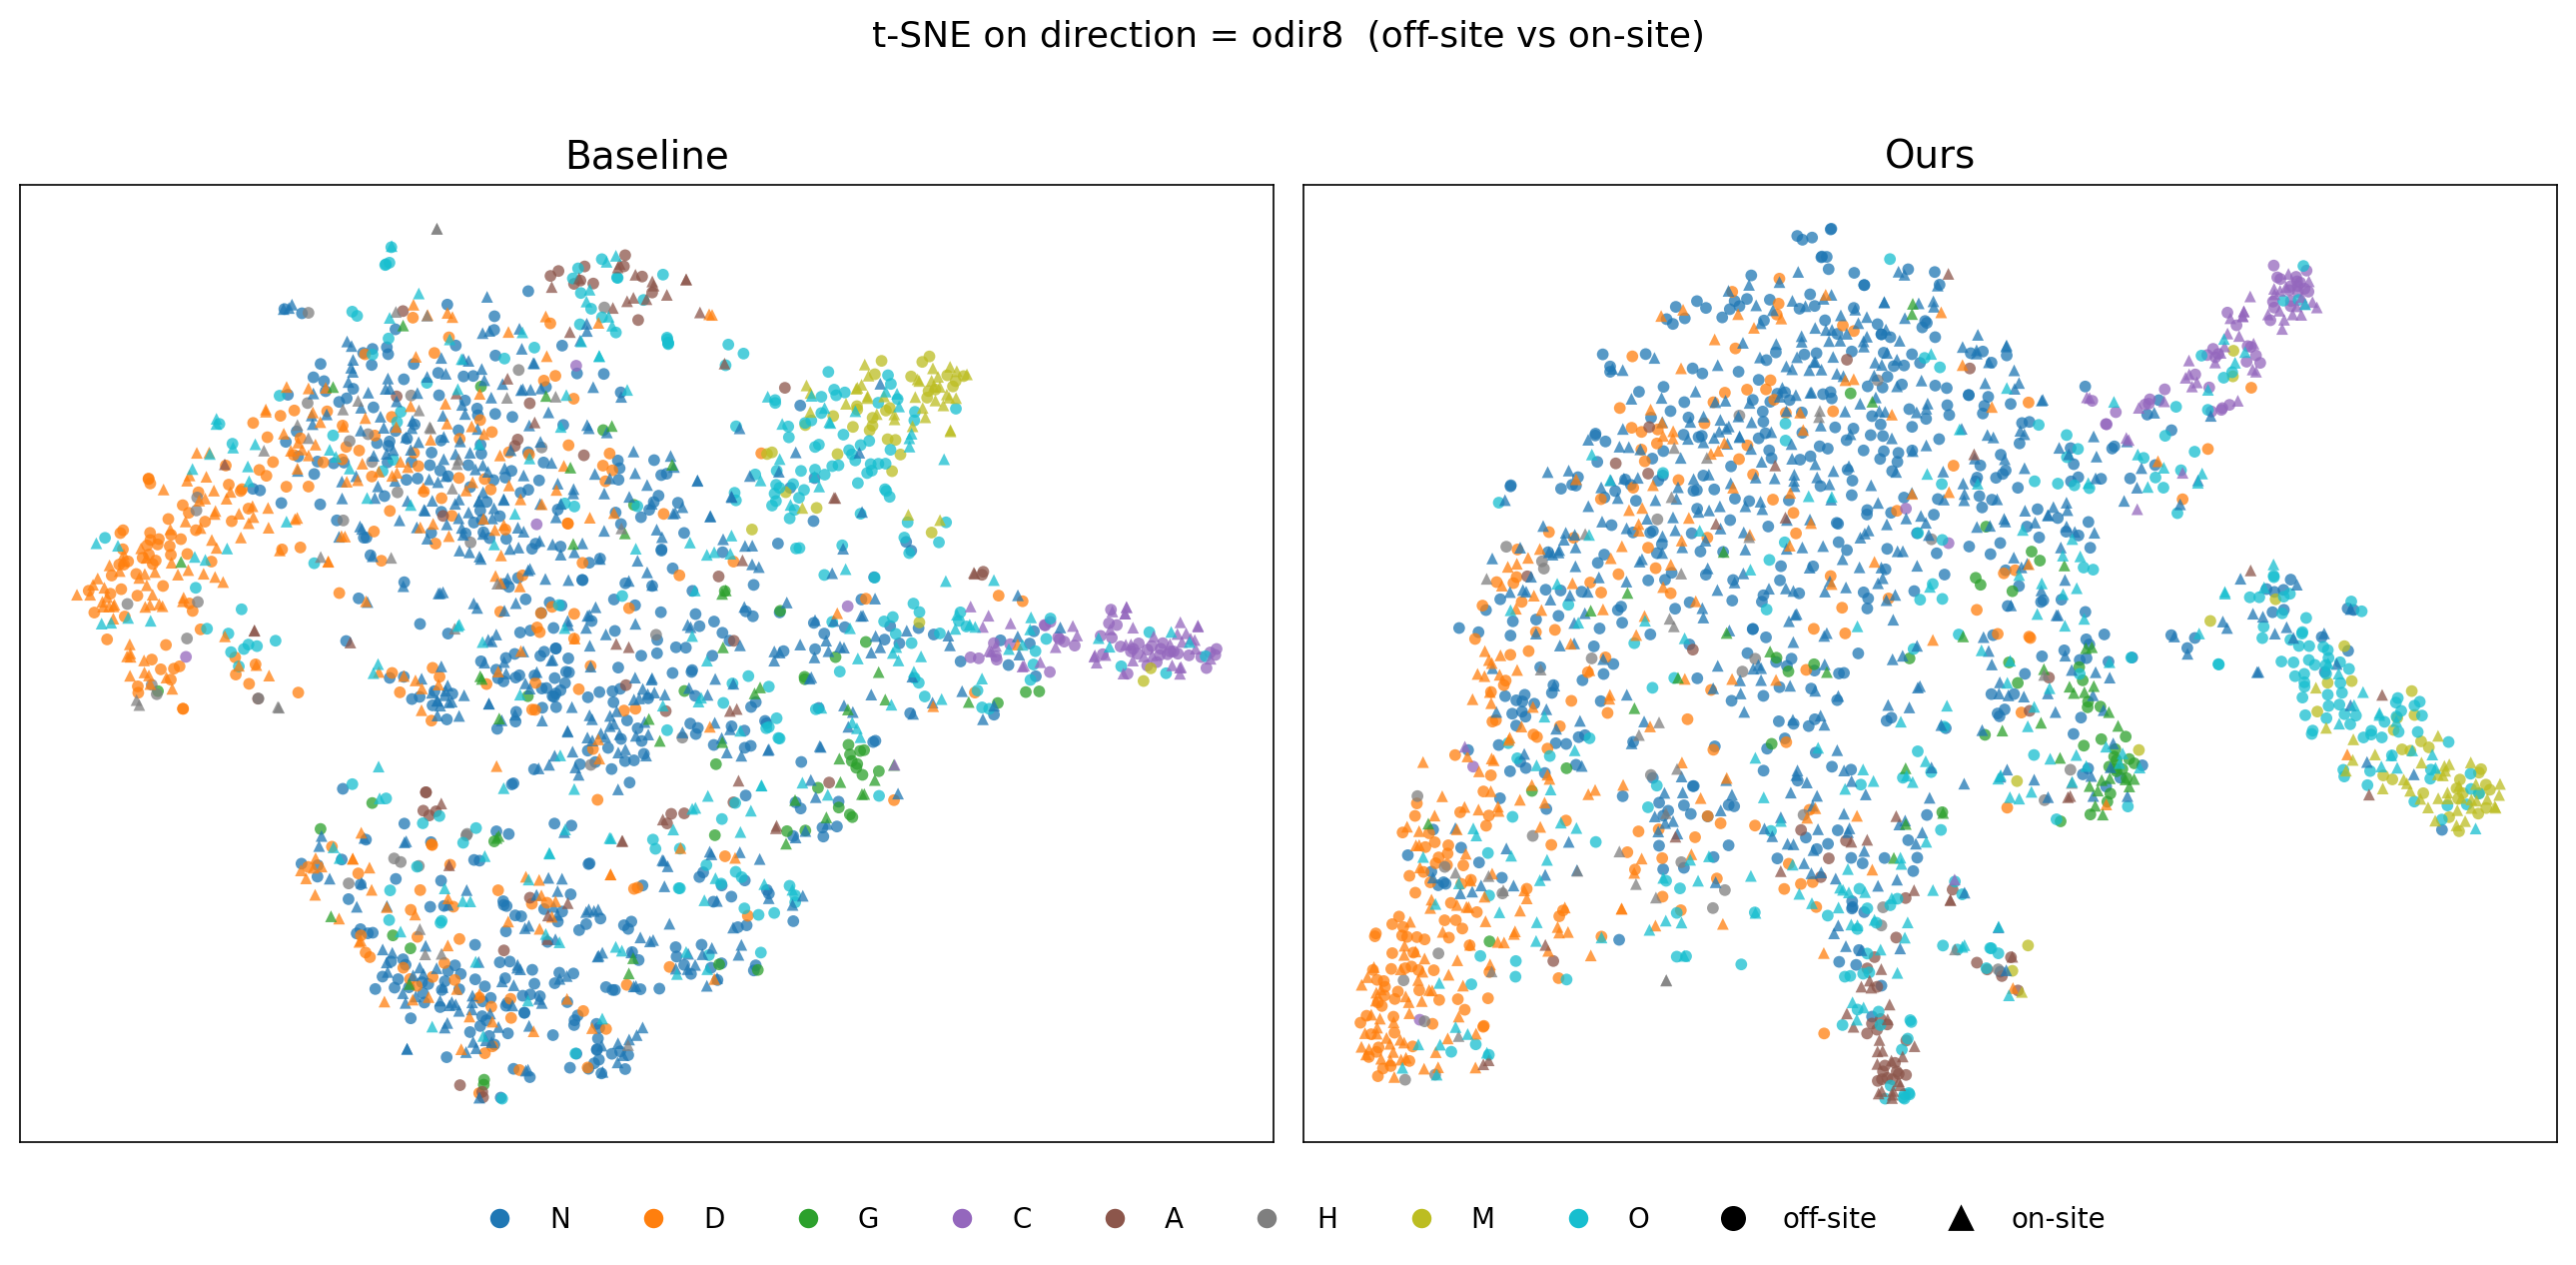
\includegraphics[width=0.60\textwidth]{./images/plots/tsne_odir8_panel1_tx.png}
\caption{ODIR Off-site \(\rightarrow\) On-site（域内泛化，8 类 / in-domain generalization, 8 classes）}
\label{fig:tsne-odir}
\end{subfigure}

\vspace{4pt}
\begin{subfigure}{\textwidth}
\centering
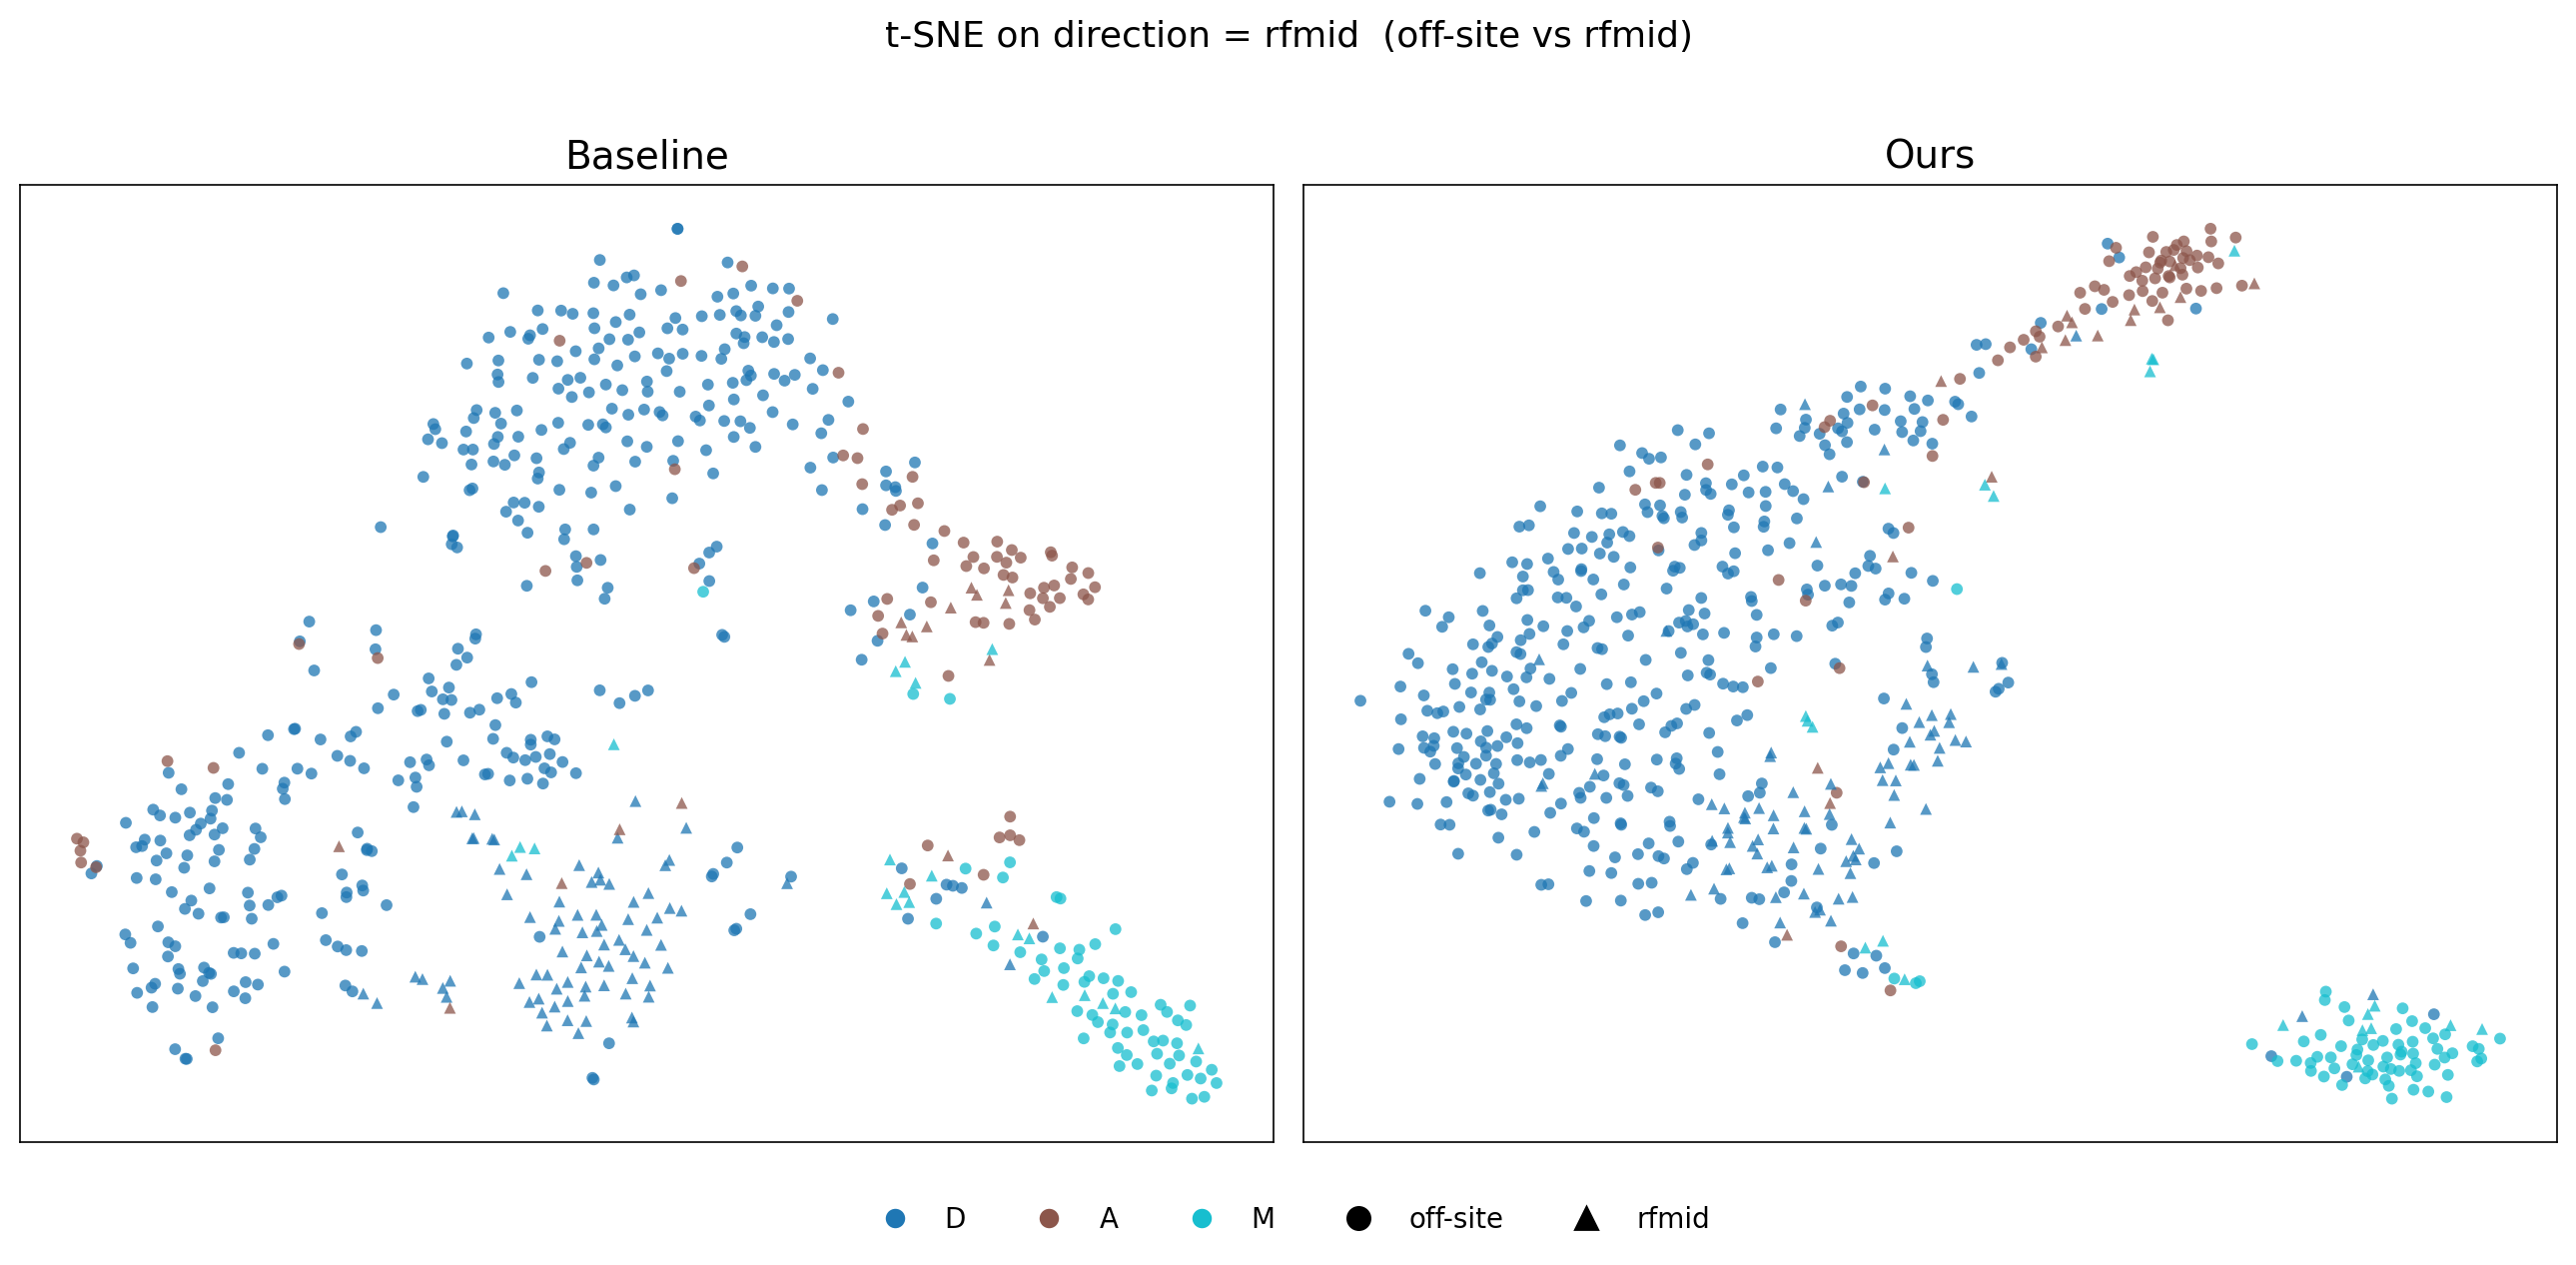
\includegraphics[width=0.60\textwidth]{./images/plots/tsne_rfmid_panel1_tx.png}
\caption{ODIR Off-site \(\rightarrow\) RFMiD（D/A/M 三类对齐 / D/A/M three-class alignment）}
\label{fig:tsne-rfmid}
\end{subfigure}

\vspace{4pt}
\begin{subfigure}{\textwidth}
\centering
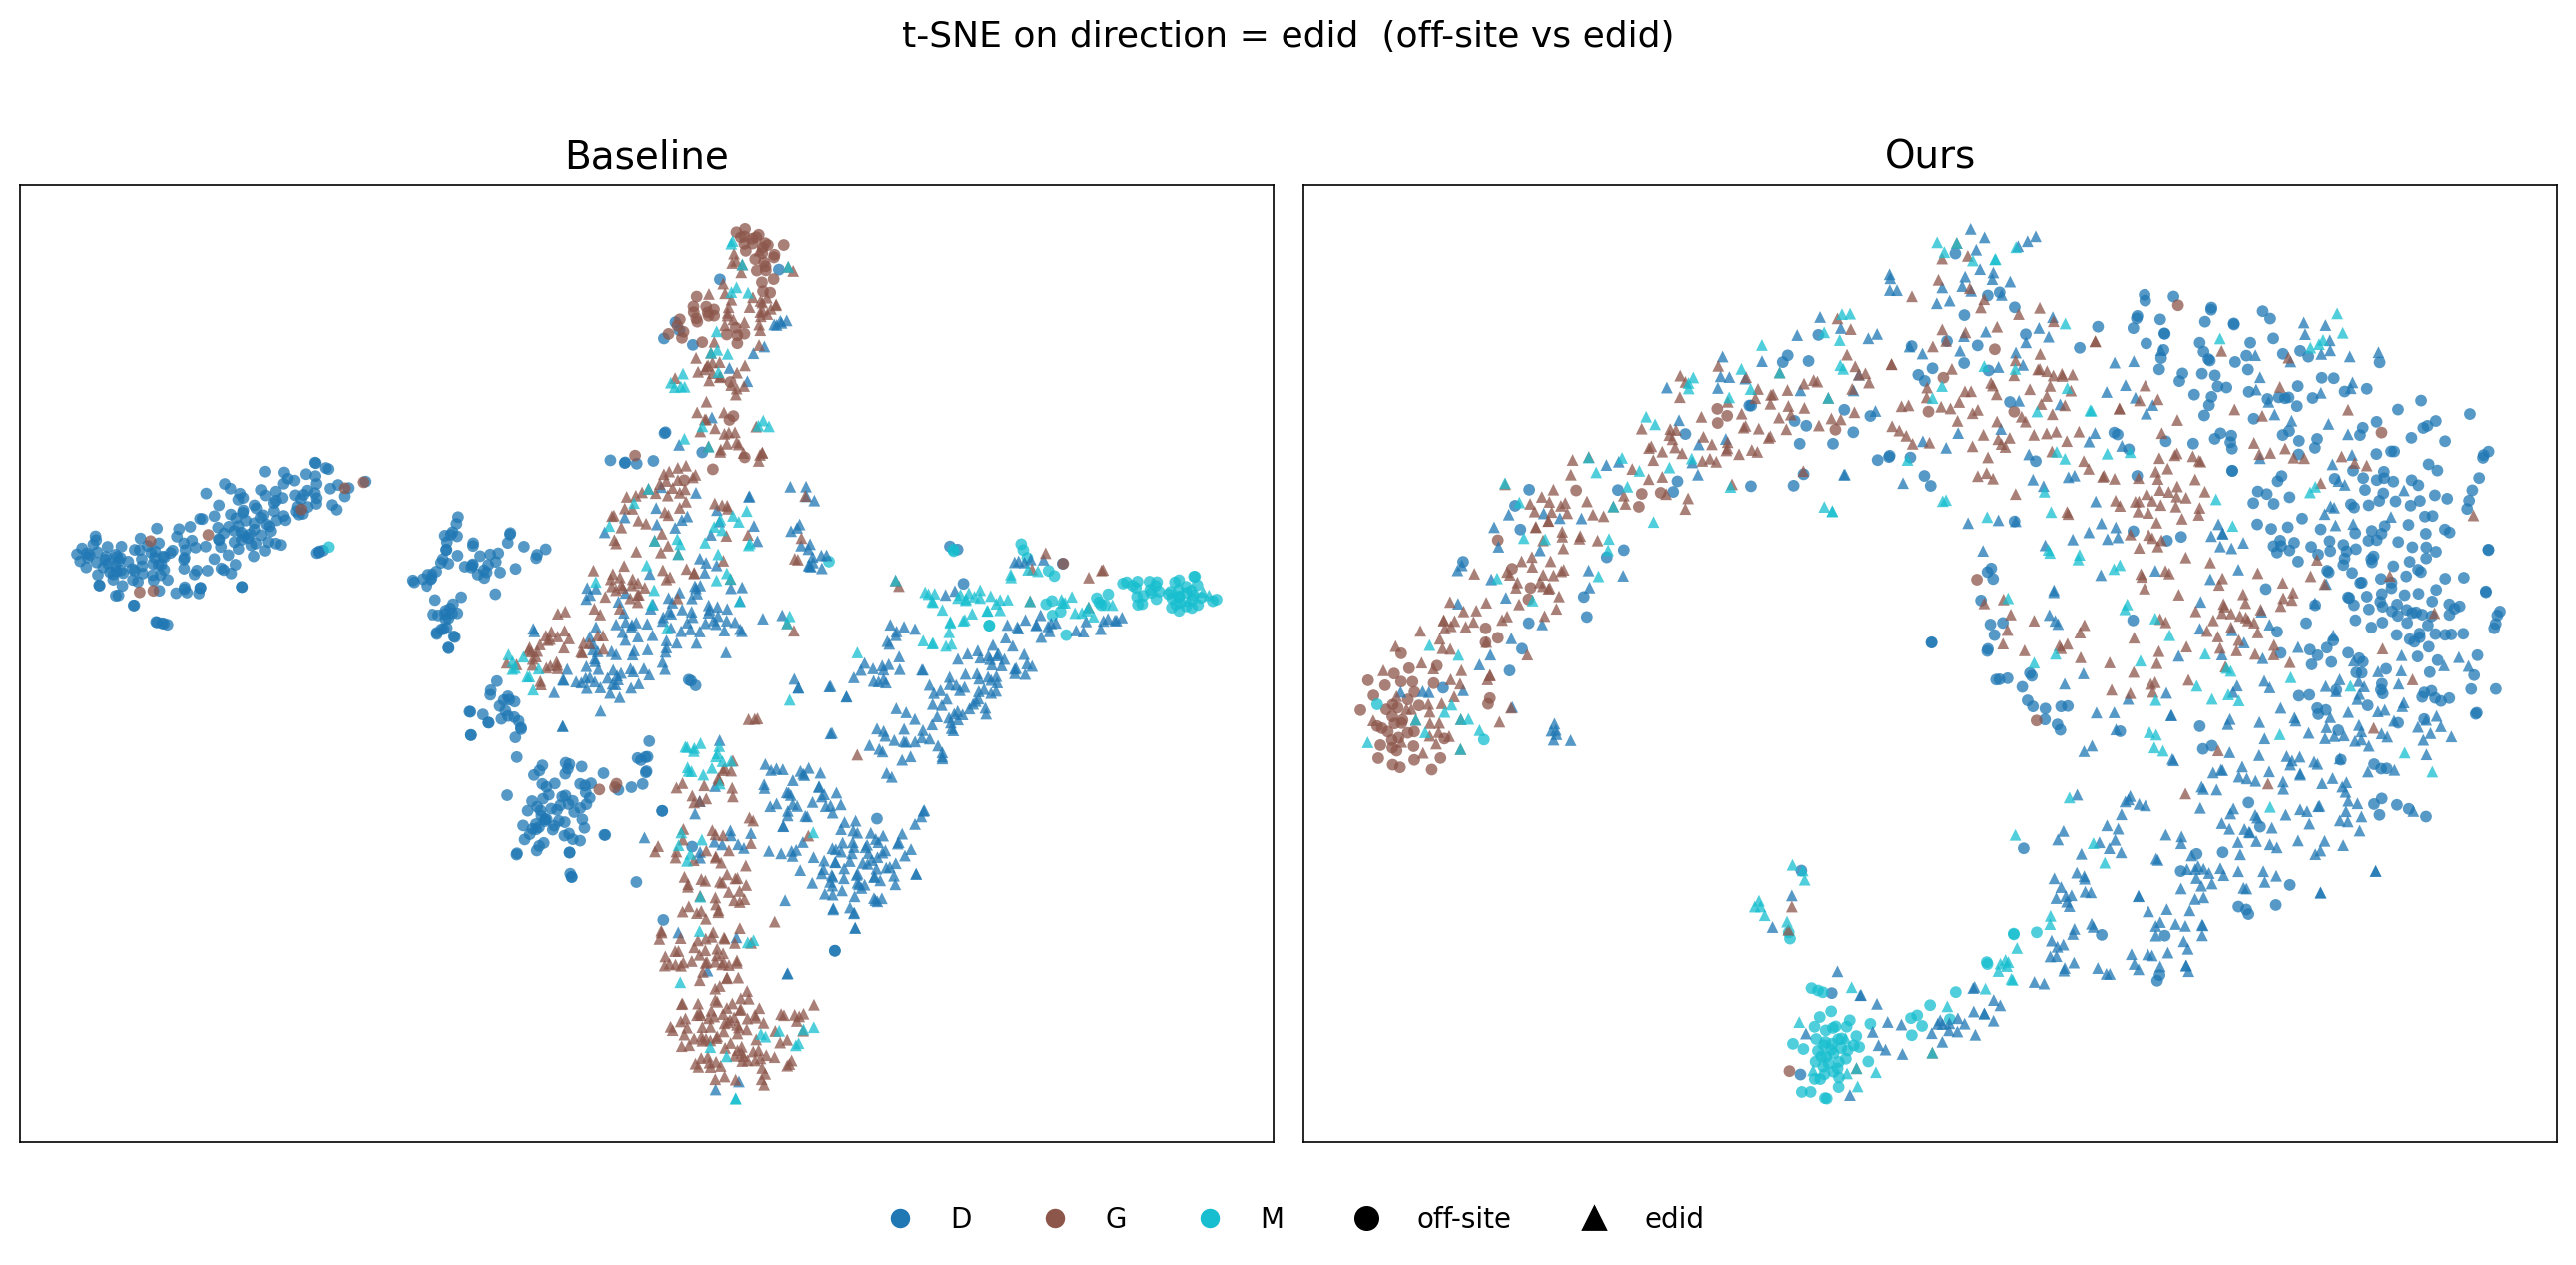
\includegraphics[width=0.60\textwidth]{./images/plots/tsne_edid_panel1_tx.png}
\caption{ODIR Off-site \(\rightarrow\) EDID（D/G/M 三类对齐 / D/G/M three-class alignment）}
\label{fig:tsne-edid}
\end{subfigure}
\captionsetup{font=small}
\caption{三个评估方向下目标域样本特征的 t-SNE 可视化，(a)--(c) 分别对应 ODIR 域内（Off-site \(\rightarrow\) On-site）、ODIR \(\rightarrow\) RFMiD 与 ODIR \(\rightarrow\) EDID 三个泛化方向。每个子图内部左侧为 baseline、右侧为所提方法（Ours），不同颜色代表不同类别，圆点为源域样本、三角为目标域样本。(a) 域内 Off-site 与 On-site 同源、域差异本身较小，两种方法的同类样本均合理重叠，Ours 在小样本疾病类（G、A、M）上呈现更清晰的局部簇结构。(b) 在 RFMiD 泛化设置下，Ours 将 D/A/M 三类组织为更独立的簇，且每个簇内源域与目标域同类样本紧密混合，而 baseline D 类内部存在多个分离子簇，三类局部聚集相对松散。(c) 在 EDID 泛化设置下，baseline 虽形成多个局部簇，但某些同一疾病类的源域与目标域样本各自聚成相邻但分离的子簇（如 D 类和 G 类存在明显的两域边界）；Ours 簇数虽有所减少，但其将同类的两域样本更加混合，大致形成 D/G/M 三个按类别（而非按域）组织的区域。最终结果证明，所提方法有更强的域泛化能力。 t-SNE visualization of target-domain sample features under three evaluation directions, where (a)--(c) correspond to ODIR in-domain (Off-site \(\rightarrow\) On-site), ODIR \(\rightarrow\) RFMiD, and ODIR \(\rightarrow\) EDID, respectively. In each subfigure, the left side is the baseline and the right side is the proposed method (Ours); different colors denote different classes, dots denote source-domain samples, and triangles denote target-domain samples. (a) In-domain Off-site and On-site share the same source and the domain gap itself is small, so same-class samples of both methods overlap reasonably, and Ours shows clearer local cluster structures on the small-sample disease classes (G, A, M). (b) Under the RFMiD generalization setting, Ours organizes the D/A/M classes into more independent clusters, with source- and target-domain samples of the same class closely mixed within each cluster, whereas the baseline has multiple separated sub-clusters within class D and looser local aggregation of the three classes. (c) Under the EDID generalization setting, the baseline also forms several local clusters, but for some classes the source- and target-domain samples of the same disease aggregate into adjacent but separated sub-clusters (for example, classes D and G show a clear two-domain boundary); Ours yields fewer clusters but mixes the two-domain samples of the same class more thoroughly, roughly forming three regions organized by class (D/G/M) rather than by domain. These results demonstrate that the proposed method has stronger domain generalization capability.}
\label{fig:tsne}
\end{figure}

2. 自适应高斯差分隐私超参数扫描 结果如\tabref{tab:privacy-scan}所示。引入隐私保护后，噪声注入速率会一定程度影响模型收敛行为与最终性能。实验发现，噪声乘数（noise\_multiplier）与噪声衰减速率（noise\_decay\_rate）共同决定了每轮噪声注入速率，并进一步影响每轮隐私预算消耗：过强的初始噪声会导致训练剧烈震荡甚至不收敛，而过快的衰减则使隐私预算在模型尚未充分学习时提前耗尽。其中，setting1（noise\_multiplier=0.65）提供了极强的隐私保护，但因初始噪声过大，导致\(\epsilon\)值仅为5.01，使模型性能严重下降；setting8（noise\_multiplier=0.25，decay\_rate=4e-6）虽然使得模型性能接近非隐私保护条件，但是\(\epsilon \approx 20\)隐私保护弱。综合性能与隐私预算，我们最终选取 setting5（noise\_multiplier=0.35，decay\_rate=4e-6），在80 epoch 后\(\epsilon \approx 10.15\)，实现了较优的隐私-性能平衡。

\begin{sloppypar}
2. Hyperparameter scan of Adaptive Gaussian Differential Privacy. The results are shown in \hyperref[tab:privacy-scan]{Table~\ref*{tab:privacy-scan}}. After introducing privacy preservation, the noise injection rate affects model convergence behavior and final performance. The experiments show that the noise multiplier and noise decay rate jointly determine the per-epoch noise injection rate and further affect privacy budget consumption in each epoch. Excessive initial noise causes severe training oscillation or even non-convergence, whereas overly fast decay exhausts the privacy budget before the model has learned sufficiently. Setting 1 (noise\_multiplier=0.65) provides very strong privacy preservation, but the excessive initial noise yields \(\epsilon=5.01\) and severely degrades model performance. Setting 8 (noise\_multiplier=0.25, noise\_decay\_rate=4e\mbox{-}6) brings model performance close to the non-private setting, but \(\epsilon \approx 20\) indicates weak privacy preservation. Considering both performance and privacy budget, we finally select Setting 5 (noise\_multiplier=0.35, noise\_decay\_rate=4e\mbox{-}6), which reaches \(\epsilon \approx 10.15\) after 80 epochs and achieves a better privacy-performance trade-off.
\end{sloppypar}

% Chapter 4 Experiments - Table 5
% Hyperparameter scan for adaptive Gaussian differential privacy.
\begin{table}[!htb]
\centering
\caption{自适应高斯差分隐私超参数扫描结果。表中比较了不同噪声乘数与噪声衰减速率组合在 80 epoch 差分隐私训练设置下对应的隐私预算 $\epsilon$。其中，setting1 下噪声注入较强，虽然隐私保护更好，但模型性能下滑较大；setting8 下噪声注入相对较缓，模型性能下滑较小，但隐私保护较弱。而红色的 setting5 为本文最终采用的设置，在隐私保护与模型性能之间取得了较好平衡。 Hyperparameter scan results for Adaptive Gaussian Differential Privacy. The table compares the privacy budget $\epsilon$ under 80-epoch differential privacy training with different combinations of noise multiplier and noise decay rate. Setting 1 injects stronger noise and provides better privacy preservation, but causes a larger performance drop. Setting 8 injects relatively weaker noise and yields a smaller performance drop, but provides weaker privacy preservation. The red Setting 5 is the final setting used in this study and achieves a better balance between privacy preservation and model performance.}
\label{tab:privacy-scan}
\begin{tabular}{lccc}
\toprule
Setting & noise\_multiplier & noise\_decay\_rate & $\epsilon$ / 80 epoch \\
\midrule
setting1 & 0.65 & 1.5e-6 & 5.01 \\
setting2 & 0.50 & 2e-6 & 6.80 \\
setting3 & 0.40 & 4e-6 & 8.71 \\
setting4 & 0.35 & 2e-6 & 9.96 \\
\textcolor{red}{setting5} & \textcolor{red}{0.35} & \textcolor{red}{4e-6} & \textcolor{red}{10.15} \\
setting6 & 0.30 & 2e-6 & 11.91 \\
setting7 & 0.25 & 2e-6 & 15.11 \\
setting8 & 0.25 & 4e-6 & 20.01 \\
\bottomrule
\end{tabular}
\end{table}


3. 隐私训练过程中的\(\epsilon\)-性能演化与优化策略 结果如\tabref{tab:privacy-evolution}所示，并在\figref{fig:privacy-tradeoff}中以隐私-性能权衡曲线直观呈现。采用 setting5 的噪声速率后，我们记录了训练过程中\(\epsilon\)消耗与单目指标的逐 epoch 变化。结果显示，随着\(\epsilon\)从第0轮的0.94逐步增长至第79轮的10.15，隐私逐步消耗，模型性能持续提升，至第74轮附近达到峰值（Final=73.15）。这表明自适应衰减策略允许模型在隐私预算内充分学习。第74轮的检查点是兼具隐私保护和性能的最佳平衡点。经过大量实验验证，隐私保护条件下需对优化策略进行针对性调整：

3. \(\epsilon\)-performance evolution and optimization strategy during privacy-preserving training. The results are shown in \hyperref[tab:privacy-evolution]{Table~\ref*{tab:privacy-evolution}} and are intuitively presented as a privacy-performance trade-off curve in \hyperref[fig:privacy-tradeoff]{Fig.~\ref*{fig:privacy-tradeoff}}. After adopting the noise rate of Setting 5, we record epoch-by-epoch changes in \(\epsilon\) consumption and monocular metrics during training. As \(\epsilon\) increases from 0.94 at epoch 0 to 10.15 at epoch 79, the privacy budget is progressively spent and model performance improves, reaching a peak around epoch 74 (Final=73.15). This indicates that the adaptive decay strategy allows the model to learn sufficiently within the privacy budget. The checkpoint at epoch 74 provides the best balance between privacy preservation and performance. Extensive experiments show that the optimization strategy needs to be adjusted for privacy-preserving scenarios:

\input{manuscripts/compare/tables/src/table4_privacy_evolution_compare.tex}

\begin{figure}[H]
\centering
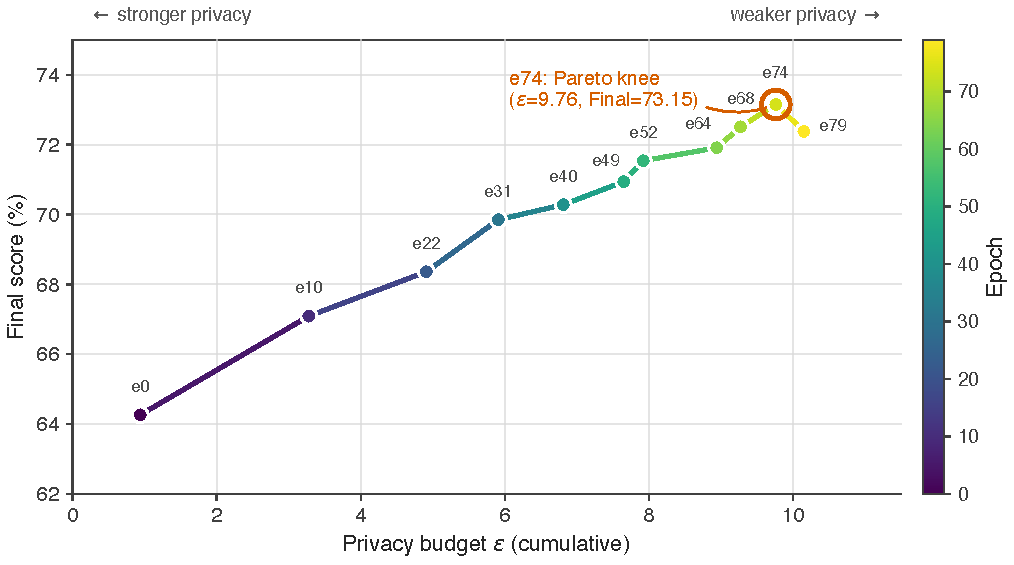
\includegraphics[width=0.78\textwidth]{./images/plots/fig_privacy_tradeoff.pdf}
\caption{隐私训练过程中的隐私-性能（\(\epsilon\)-Final score）权衡曲线，数据对应\tabref{tab:privacy-evolution}。横轴为累积隐私预算\(\epsilon\)（越靠左隐私保护越强），纵轴为单目 Final score，每个点对应一个 epoch 检查点并按训练轮次着色，轨迹展示了随训练推进的隐私-性能演化。第74轮（e74）为 Pareto 拐点，即在\(\epsilon \approx 9.76\)处取得最优 Final score（73.15），是兼顾隐私与性能的最佳工作点。 Privacy-performance (\(\epsilon\)-Final score) trade-off curve during privacy-preserving training, with data corresponding to \hyperref[tab:privacy-evolution]{Table~\ref*{tab:privacy-evolution}}. The horizontal axis is the cumulative privacy budget \(\epsilon\) (stronger privacy preservation toward the left), and the vertical axis is the monocular Final score. Each point corresponds to an epoch checkpoint and is colored by training epoch; the trajectory shows the privacy-performance evolution as training proceeds. Epoch 74 (e74) is the Pareto knee point, achieving the best Final score (73.15) at \(\epsilon \approx 9.76\), and is the best operating point that balances privacy and performance.}
\label{fig:privacy-tradeoff}
\end{figure}

（1）学习率从\(1 \times 10^{-5}\)提升至\(7.5 \times 10^{-5}\)。

(1) The learning rate is increased from \(1 \times 10^{-5}\) to \(7.5 \times 10^{-5}\).

（2）学习率调度改为``先线性衰减后恒定''： 以 lr\_decay\_ratio 和 lr\_final\_factor 控制衰减轮次和衰减比例，所取值分别为0.75和0.8，即学习率在前75\%轮次内线性衰减至原值的80\%，之后保持恒定训练。

(2) The learning-rate schedule is changed to linear decay followed by constant training. The learning rate decay ratio and final learning rate factor control the decay epochs and decay ratio, and are set to 0.75 and 0.8, respectively. That is, the learning rate linearly decays to 80\% of its original value during the first 75\% of epochs and then remains constant.

原因在于，隐私保护条件下的模型训练和非隐私保护条件下的模型训练不一样。对于学习率的取值来说，隐私保护条件下，每一次回传的梯度中都会叠加噪声，这使得每一次模型优化时的损失值在原基础上波动，增大了陷入局部最优的概率，因此学习率需要适当增大。对于学习率调度策略，在非隐私保护条件下当模型收敛到最优值附近时，学习速率通常会逐步减小；相比之下，隐私保护条件下的学习过程不需要将学习率降低到一个非常小的值，因为差分隐私训练会以隐私消耗不断增大的代价持续优化，却未必真正达到模型收敛。因此，以相对较大的学习率开始，然后在一定周期内线性衰减到较小的值，并在之后保持恒定，性能会更好。

This adjustment is motivated by the differences between privacy-preserving training and non-private training. For the learning rate, noise is added to each backpropagated gradient under privacy-preserving training, causing the loss at each optimization step to fluctuate and increasing the risk of poor local optima. A moderately larger learning rate is therefore needed. For the learning-rate schedule, non-private training usually decreases the learning rate as the model approaches an optimum. In contrast, privacy-preserving training does not need to reduce the learning rate to a very small value, because differential privacy training continues optimization while privacy loss accumulates, but may not fully converge. Starting with a relatively large learning rate, linearly decaying it to a smaller value over a certain period, and then keeping it constant therefore yields better performance.

实验证明，该策略改善了收敛稳定性，最终在\(\epsilon = 9.76\)时取得了73.15的 Final score，明显优于固定噪声或低学习率配置。

Experiments demonstrate that this strategy improves convergence stability and achieves a Final score of 73.15 at \(\epsilon = 9.76\), clearly outperforming fixed-noise or low-learning-rate configurations.

4. 隐私保护下的最终泛化性能 结果如\tabref{tab:privacy-final}所示。由于现有多标签眼科疾病识别泛化工作鲜有同时报告隐私训练下的指标，本文以 Li et al. \hyperref[_Ref213949402]{{[}46{]}} 提供的 ODIR 官方 ResNet50 基线作为公开参考点，用于评估隐私训练能否保持与公开基准相当的性能水平。最优隐私模型在 ODIR 域内双目指标上的 Off-site 和 On-site Final score 分别为68.96和68.42，相较本文非隐私保护版本下降约10个百分点；与官方基线相比，所提方法的 Off-site 略优（68.96 vs. 68.00），On-site 略低（68.42 vs. 68.80），整体保持在公开基准附近，说明在中等隐私预算下，自适应高斯差分隐私机制能够在提供有效隐私保护的同时使性能维持在可接受范围内。

4. Final generalization performance under privacy preservation. The results are shown in \hyperref[tab:privacy-final]{Table~\ref*{tab:privacy-final}}. Since existing generalization studies on multi-label ocular disease recognition rarely report metrics under privacy-preserving training, this study uses the official ODIR ResNet50 baseline provided by Li et al. \hyperref[_Ref213949402]{{[}46{]}} as a public reference point to assess whether privacy-preserving training can maintain performance comparable to a public benchmark. The optimal privacy checkpoint achieves Off-site and On-site Final scores of 68.96 and 68.42 on ODIR in-domain binocular metrics, respectively, about 10 percentage points lower than our non-private version. Compared with the official baseline, the proposed method is slightly better on Off-site (68.96 vs. 68.00) and slightly lower on On-site (68.42 vs. 68.80), remaining around the public benchmark overall. This indicates that, under a moderate privacy budget, the Adaptive Gaussian Differential Privacy mechanism can provide effective privacy preservation while keeping performance within an acceptable range.
% Chapter 4 Experiments - Table 7
% Final generalization performance under privacy mode.
\begin{table}[!htb]
\centering
\caption{隐私保护下的泛化性能对比。表中报告 ODIR 域内双目 Final score，其中 Ours（privacy）采用的是\tabref{tab:privacy-evolution}中选取的最优隐私检查点。在中等隐私预算下，所提方法在 Off-site 上略优于 Li et al. \hyperref[_Ref213949402]{{[}46{]}} 报告的官方基线，并在 On-site 上保持接近性能。 Comparison of generalization performance under privacy preservation. The table reports ODIR in-domain binocular Final score. Ours (privacy) uses the optimal privacy checkpoint selected in \tabref{tab:privacy-evolution}. Under a moderate privacy budget, the proposed method slightly outperforms the official baseline reported by Li et al. \hyperref[_Ref213949402]{{[}46{]}} on Off-site and maintains comparable performance on On-site.}
\label{tab:privacy-final}
\begin{tabular}{lcc}
\toprule
Model & Off-site & On-site \\
\midrule
Li et al. \hyperref[_Ref213949402]{{[}46{]}} & 68.00 & \textbf{68.80} \\
\textbf{Ours (privacy)} & \textbf{68.96} & 68.42 \\
\bottomrule
\end{tabular}
\end{table}

